%definira klasu dokumenta 
\documentclass[12pt]{report} 

%prostor izmedu naredbi \documentclass i \begin{document} se zove uvod. U njemu se nalaze naredbe koje se odnose na cijeli dokument

%osnovni LaTex ne može riješiti sve probleme, pa se koriste različiti paketi koji olakšavaju izradu željenog dokumenta
\usepackage[croatian]{babel} 
\usepackage{amssymb}
\usepackage{amsmath}
\usepackage{txfonts}
\usepackage{mathdots}
\usepackage{titlesec}
\usepackage{array}
\usepackage{lastpage}
\usepackage{etoolbox}
\usepackage{tabularray}
\usepackage{color, colortbl}
\usepackage{adjustbox}
\usepackage{geometry}
\usepackage[classicReIm]{kpfonts}
\usepackage{hyperref}
\usepackage{fancyhdr}

\usepackage{float}
\usepackage{setspace}
\restylefloat{table}


\patchcmd{\chapter}{\thispagestyle{plain}}{\thispagestyle{fancy}}{}{} %redefiniranje stila stranice u paketu fancyhdr

%oblik naslova poglavlja
\titleformat{\chapter}{\normalfont\huge\bfseries}{\thechapter.}{20pt}{\Huge}
\titlespacing{\chapter}{0pt}{0pt}{40pt}


\linespread{1.3} %razmak između redaka

\geometry{a4paper, left=1in, top=1in,}  %oblik stranice

\hypersetup{ colorlinks, citecolor=black, filecolor=black, linkcolor=black,	urlcolor=black }   %izgled poveznice


%prored smanjen između redaka u nabrajanjima i popisima
\newenvironment{packed_enum}{
	\begin{enumerate}
		\setlength{\itemsep}{0pt}
		\setlength{\parskip}{0pt}
		\setlength{\parsep}{0pt}
	}{\end{enumerate}}

\newenvironment{packed_item}{
	\begin{itemize}
		\setlength{\itemsep}{0pt}
		\setlength{\parskip}{0pt}
		\setlength{\parsep}{0pt}
	}{\end{itemize}}




%boja za privatni i udaljeni kljuc u tablicama
\definecolor{LightBlue}{rgb}{0.9,0.9,1}
\definecolor{LightGreen}{rgb}{0.9,1,0.9}

%Promjena teksta za dugačke tablice
\DefTblrTemplate{contfoot-text}{normal}{Nastavljeno na idućoj stranici}
\SetTblrTemplate{contfoot-text}{normal}
\DefTblrTemplate{conthead-text}{normal}{(Nastavljeno)}
\SetTblrTemplate{conthead-text}{normal}
\DefTblrTemplate{middlehead,lasthead}{normal}{Nastavljeno od prethodne stranice}
\SetTblrTemplate{middlehead,lasthead}{normal}

%podesavanje zaglavlja i podnožja

\pagestyle{fancy}
\lhead{Programsko inženjerstvo}
\rhead{$<$Projektni zadatak$>$}
\lfoot{$<$Naziv grupe$>$}
\cfoot{stranica \thepage/\pageref{LastPage}}
\rfoot{\today}
\renewcommand{\headrulewidth}{0.2pt}
\renewcommand{\footrulewidth}{0.2pt}


\begin{document} 
	
	
	
	\begin{titlepage}
		\begin{center}
			\vspace*{\stretch{1.0}} %u kombinaciji s ostalim \vspace naredbama definira razmak između redaka teksta
			\LARGE Programsko inženjerstvo\\
			\large Ak. god. 2023./2024.\\
			
			\vspace*{\stretch{3.0}}
			
			\huge {Sustav za prijavu oštećenja javnih površina (name subject to change)\\}
			\Large Dokumentacija, Rev. \textit{$<$1 ili 2$>$}\\
			
			\vspace*{\stretch{12.0}}
			\normalsize
			Grupa: \textit{VelicanstveniTimRaketa}\\
			Koordinator: \textit{Ivan Šimunić}\\
			
			
			\vspace*{\stretch{1.0}}
			Datum predaje: \textit{$<$dan$>$. $<$mjesec$>$. $<$godina$>$.}\\
	
			\vspace*{\stretch{4.0}}
			
			Nastavnik: \textit{Izv. prof. dr. sc. Vlado Sruk}\\
		
		\end{center}

	
	\end{titlepage}

	
	\tableofcontents


	\chapter{Dnevnik promjena dokumentacije}
		
		\textbf{\textit{Kontinuirano osvježavanje}}\\
				
		
		\begin{longtblr}[
				label=none
			]{
				width = \textwidth, 
				colspec={|X[2]|X[13]|X[3]|X[3]|}, 
				rowhead = 1
			}
			\hline
			\textbf{Rev.}	& \textbf{Opis promjene/dodatka} & \textbf{Autori} & \textbf{Datum}\\[3pt] \hline
			0.1 & Napravljen predložak.	& Ivan Šimunić & 26.10.2023. 		\\[3pt] \hline 
			verzija	& što je novo \newline napravljeno/dodano. & autori & datum 	\\[3pt] \hline 
			0.2	& Dopisane upute za povijest dokumentacije.\newline Dodane reference. & * & 24.08.2013. 	\\[3pt] \hline 
			0.5 & Dodan \textit{Use Case} dijagram i jedan sekvencijski dijagram, funkcionalni i nefunkcionalni zahtjevi i dodatak A & * & 25.08.2013. \\[3pt] \hline 
			0.6 & Arhitektura i dizajn sustava, algoritmi i strukture podataka & * & 26.08.2013. \\[3pt] \hline 
			0.8 & Povijest rada i trenutni status implementacije,\newline Zaključci i plan daljnjeg rada & * & 28.08.2013. \\[3pt] \hline 
			0.9 & Opisi obrazaca uporabe & * & 07.09.2013. \\[3pt] \hline 
			0.10 & Preveden uvod & * & 08.09.2013. \\[3pt] \hline 
			0.11 & Sekvencijski dijagrami & * & 09.09.2013. \\[3pt] \hline 
			0.12.1 & Započeo dijagrame razreda & * & 10.09.2013. \\[3pt] \hline 
			0.12.2 & Nastavak dijagrama razreda & * & 11.09.2013. \\[3pt] \hline 
			\textbf{1.0} & Verzija samo s bitnim dijelovima za 1. ciklus & * & 11.09.2013. \\[3pt] \hline 
			1.1 & Uređivanje teksta -- funkcionalni i nefunkcionalni zahtjevi & * \newline * & 14.09.2013. \\[3pt] \hline 
			1.2 & Manje izmjene:Timer - Brojilo vremena & * & 15.09.2013. \\[3pt] \hline 
			1.3 & Popravljeni dijagrami obrazaca uporabe & * & 15.09.2013. \\[3pt] \hline 
			1.5 & Generalna revizija strukture dokumenta & * & 19.09.2013. \\[3pt] \hline 
			1.5.1 & Manja revizija (dijagram razmještaja) & * & 20.09.2013. \\[3pt] \hline 
			\textbf{2.0} & Konačni tekst predloška dokumentacije  & * & 28.09.2013. \\[3pt] \hline 
			&  &  & \\[3pt] \hline	
		\end{longtblr}
	
	
		\textit{Moraju postojati glavne revizije dokumenata 1.0 i 2.0 na kraju prvog i drugog ciklusa. Između tih revizija mogu postojati manje revizije već prema tome kako se dokument bude nadopunjavao. Očekuje se da nakon svake značajnije promjene (dodatka, izmjene, uklanjanja dijelova teksta i popratnih grafičkih sadržaja) dokumenta se to zabilježi kao revizija. Npr., revizije unutar prvog ciklusa će imati oznake 0.1, 0.2, …, 0.9, 0.10, 0.11.. sve do konačne revizije prvog ciklusa 1.0. U drugom ciklusu se nastavlja s revizijama 1.1, 1.2, itd.}
	\chapter{Opis projektnog zadatka}
		
		\textbf{\textit{dio 1. revizije}}\\
		
		\textit{Na osnovi projektnog zadatka detaljno opisati korisničke zahtjeve. Što jasnije opisati cilj projektnog zadatka, razraditi problematiku zadatka, dodati nove aspekte problema i potencijalnih rješenja. Očekuje se minimalno 3, a poželjno 4-5 stranica opisa.	Teme koje treba dodatno razraditi u ovom poglavlju su:}
		\begin{packed_item}
			\item \textit{potencijalna korist ovog projekta}
			\item \textit{postojeća slična rješenja (istražiti i ukratko opisati razlike u odnosu na zadani zadatak). Dodajte slike koja predočavaju slična rješenja.}
			\item \textit{skup korisnika koji bi mogao biti zainteresiran za ostvareno rješenje.}
			\item \textit{mogućnost prilagodbe rješenja }
			\item \textit{opseg projektnog zadatka}
			\item \textit{moguće nadogradnje projektnog zadatka}
		\end{packed_item}
		
		\textit{Za pomoć pogledati reference navedene u poglavlju „Popis literature“, a po potrebi konzultirati sadržaj na internetu koji nudi dobre smjernice u tom pogledu.}
		\eject
		
		\section{Primjeri u \LaTeX u}
		
		\textit{Ovo potpoglavlje izbrisati.}\\

		U nastavku se nalaze različiti primjeri kako koristiti osnovne funkcionalnosti \LaTeX a koje su potrebne za izradu dokumentacije. Za dodatnu pomoć obratiti se asistentu na projektu ili potražiti upute na sljedećim web sjedištima:
		\begin{itemize}
			\item Upute za izradu diplomskog rada u \LaTeX u - \url{https://www.fer.unizg.hr/_download/repository/LaTeX-upute.pdf}
			\item \LaTeX\ projekt - \url{https://www.latex-project.org/help/}
			\item StackExchange za Tex - \url{https://tex.stackexchange.com/}\\
		
		\end{itemize} 	


		
		\noindent \underbar{podcrtani tekst}, \textbf{podebljani tekst}, 	\textit{nagnuti tekst}\\
		\noindent \normalsize primjer \large primjer \Large primjer \LARGE {primjer} \huge {primjer} \Huge primjer \normalsize
				
		\begin{packed_item}
			
			\item  primjer
			\item  primjer
			\item  primjer
			\item[] \begin{packed_enum}
				\item primjer
				\item[] \begin{packed_enum}
					\item[1.a] primjer
					\item[b] primjer
				\end{packed_enum}
				\item primjer
			\end{packed_enum}
			
		\end{packed_item}
		
		\noindent primjer url-a: \url{https://www.fer.unizg.hr/predmet/proinz/projekt}
		
		\noindent posebni znakovi: \# \$ \% \& \{ \} \_ 
		$|$ $<$ $>$ 
		\^{} 
		\~{} 
		$\backslash$ 
		
		
		\begin{longtblr}[
			label=none,
			entry=none
			]{
				width = \textwidth,
				colspec={|X[8,l]|X[8, l]|X[16, l]|}, 
				rowhead = 1,
			} %definicija širine tablice, širine stupaca, poravnanje i broja redaka naslova tablice
			\hline \SetCell[c=3]{c}{\textbf{naslov unutar tablice}}	 \\ \hline[3pt]
			\SetCell{LightGreen}IDKorisnik & INT	&  	Lorem ipsum dolor sit amet, consectetur adipiscing elit, sed do eiusmod  	\\ \hline
			korisnickoIme	& VARCHAR &   	\\ \hline 
			email & VARCHAR &   \\ \hline 
			ime & VARCHAR	&  		\\ \hline 
			\SetCell{LightBlue} primjer	& VARCHAR &   	\\ \hline 
		\end{longtblr}
		

		\begin{longtblr}[
				caption = {Naslov s referencom izvan tablice},
				entry = {Short Caption},
			]{
				width = \textwidth, 
				colspec = {|X[8,l]|X[8,l]|X[16,l]|}, 
				rowhead = 1,
			}
			\hline
			\SetCell{LightGreen}IDKorisnik & INT	&  	Lorem ipsum dolor sit amet, consectetur adipiscing elit, sed do eiusmod  	\\ \hline
			korisnickoIme	& VARCHAR &   	\\ \hline 
			email & VARCHAR &   \\ \hline 
			ime & VARCHAR	&  		\\ \hline 
			\SetCell{LightBlue} primjer	& VARCHAR &   	\\ \hline 
		\end{longtblr}
	


		
		
		%unos slike
		\begin{figure}[H]
			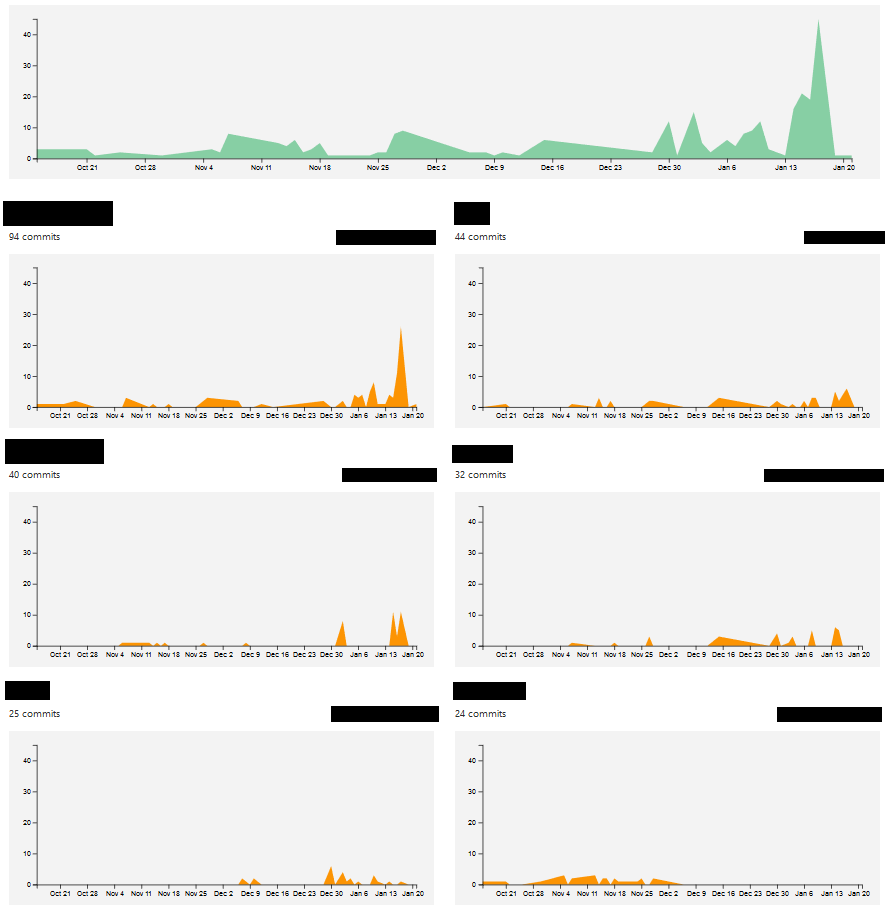
\includegraphics[scale=0.4]{slike/aktivnost.PNG} %veličina slike u odnosu na originalnu datoteku i pozicija slike
			\centering
			\caption{Primjer slike s potpisom}
			\label{fig:promjene}
		\end{figure}
		
		\begin{figure}[H]
			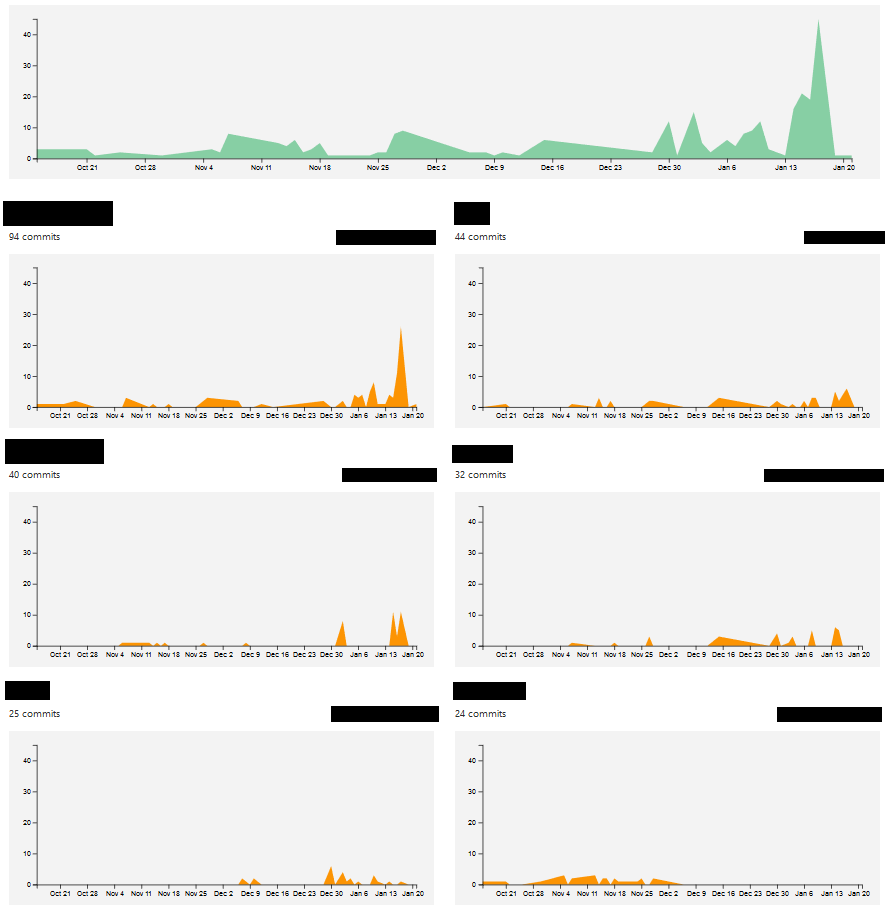
\includegraphics[width=\textwidth]{slike/aktivnost.PNG} %veličina u odnosu na širinu linije
			\caption{Primjer slike s potpisom 2}
			\label{fig:promjene2} %label mora biti drugaciji za svaku sliku
		\end{figure}
		
		Referenciranje slike \ref{fig:promjene2} u tekstu.
		
		\eject
		
	
	\chapter{Specifikacija programske potpore}
		
	\section{Funkcionalni zahtjevi}
			
			\noindent \textbf{Dionici:}
			
			\begin{packed_enum}
				
				\item Regitrirani korisnik
					\begin{packed_enum}
						\item Klijent
						\item Administrator
					\end{packed_enum}
				\item Neregistrirani (anonimni) korisnik
				\item Razvojni tim
				\item Gradski ured
				
			\end{packed_enum}
			
			\noindent \textbf{Aktori i njihovi funkcionalni zahtjevi:}
			
			
			\begin{packed_enum}
				\item  \underbar{Klijent (inicijator) može:}
				
				\begin{packed_enum}
					
					\item Prijaviti se u sustav koristeći svoj email i lozinku
					\item Odjaviti se iz sustava
					\item Pregledati osobne podatke
					\item Mijenjati osobne podatke
					\item Izbrisati svoj profil
					\item Podnijeti prijavu preko web sučelja koja sadrži naziv, opis, geografske koordinate, te opcionalno fotografiju
					\item Odabrati koordinate preko karte ili unijeti najbližu adresu
					\item Povezati svoju prijavu na postojeću (ako takva postoji)
					\item Vidjeti promjene u statusu svoje prijave
					\item Odabrati aktivne prijave na karti
					\item Imati uvid u sve prijave u sustavu
					\item Pregledati povijet svojih prijava
					\item Filtrirati pregled prijava po lokaciji i temi
					\item Mijenjati podatke aktivne prijave u povijesti prijava
				\end{packed_enum}
				
				\pagebreak
			
				\item  \underbar{Administrator (inicijator) može:}
				
				\begin{packed_enum}
					
					\item Imati uvid u popis svih prijava
					\item Imati uvid u popis svih registriranih profila
					\item Uređivati podatke prijava
					\item Brisati prijave
					\item Imati uvid u popis svih gradskih ureda
					\item Uklanjati (brisati) korisničke profile
				\end{packed_enum}
				
				\item  \underbar{Neregistrirani korisnik (incijator) može:}
				
				\begin{packed_enum}
					\item Napraviti novi korisnički račun klijenta (registrirati se u sustav)
					\item Podnijeti prijavu preko web sučelja koja sadrži naziv, opis, geografske koordinate, te opcionalno fotografiju
					\item Odabrati koordinate preko karte ili unijeti najbližu adresu
					\item Povezati svoju prijavu na postojeću (ako takva postoji)
					\item Imati uvid u sve prijave na stranici, te iste grupirati po temi i lokaciji

				\end{packed_enum}
				
				\item  \underbar{Baza podataka (sudionik) može:}
				
				\begin{packed_enum}
				\item Imati popis svih postojećih korisničkih računa
				\item Sadržavati sve jedinstvene oznake prijava neregistriranih oznaka
				\item Pohraniti svaku prijavu
					
				\end{packed_enum}
			\end{packed_enum}
			\eject 
			
			
				
			\subsection{Obrasci uporabe}
				
				\textbf{\textit{dio 1. revizije}}
				
				\subsubsection{Opis obrazaca uporabe}
					

					\noindent \underbar{\textbf{UC01 - Registracija korisnika u sustav}}
					\begin{packed_item}
	
						\item \textbf{Glavni sudionik: }Neregistrirani korisnik
						\item  \textbf{Cilj:} Stvoriti korisnički račun
						\item  \textbf{Sudionici:} Baza podataka
						\item  \textbf{Preduvjet:} Null
						\item  \textbf{Opis osnovnog tijeka:}
						
						\item[] \begin{packed_enum}
	
							\item Klijent bira opciju "registracija" na sučelju web aplikacicje
							\item Klijent unosi tažene podatke
							\item Korisnik je upisan u bazu podataka
						\end{packed_enum}
						
						\item  \textbf{Opis mogućih odstupanja:}
						
						\item[] \begin{packed_item}
	
							\item[2.a] Klijent unosi neispravni/postojeći username ili email
							\item[] \begin{packed_enum}
								
								\item Sustav obavještava korisnika o problemu i briše mu unesena polja
								
								\item Korisnik mijenja podatke u ispravne i registracija uspješno se privede kraju
								
							\end{packed_enum}
							
						\end{packed_item}
					\end{packed_item}
					
					\noindent \underbar{\textbf{UC02 - Unos nove prijave u sustav}}
					\begin{packed_item}
	
						\item \textbf{Glavni sudionik: }Korisnik
						\item  \textbf{Cilj:} Podnijeti novu prijavu
						\item  \textbf{Sudionici:} Baza podataka
						\item  \textbf{Preduvjet:} Null
						\item  \textbf{Opis osnovnog tijeka:}
						
						\item[] \begin{packed_enum}
	
							\item Korisnik upisuje tražene podatke pri unosu prijave 
							\item Sustav javlja ako postoji vremenski bliska prijava na toj lokaciji
							\item Korisnik može povezati svoju prijavu na postojeću (ako takva postoji)
							\item Prijava se predaje i zapisuje u sustav
						\end{packed_enum}
						
						\item  \textbf{Opis mogućih odstupanja:}
						
						\item[] \begin{packed_item}
	
							\item[1.a] Korisnik nije naveo sve zahtijevane podatke
							\item[] \begin{packed_enum}
								
								\item Sustav obavještava korisnika o problemu i javlja mu da popuni tražena polja
								
							\end{packed_enum}
							
						\end{packed_item}
					\end{packed_item}
					
					\pagebreak
					
					\noindent \underbar{\textbf{UC03 - Pregled prijava}}
					\begin{packed_item}
	
						\item \textbf{Glavni sudionik: }Korisnik
						\item  \textbf{Cilj:} Pregled postojećih prijava
						\item  \textbf{Sudionici:} Baza podataka
						\item  \textbf{Preduvjet:} Null
						\item  \textbf{Opis osnovnog tijeka:}
						
						\item[] \begin{packed_enum}
	
							\item Korisnik otvara pregled svih postojećih prijava
							\item Korisniku se nudi opcija filtriranja po temi i lokaciji
							\item Na sučelju se prikazuju filtritrane prijave
						\end{packed_enum}
					\end{packed_item}
					
					\noindent \underbar{\textbf{UC04 - Prijava u sustav}}
					\begin{packed_item}
	
						\item \textbf{Glavni sudionik: }Registrirani korisnik
						\item  \textbf{Cilj:} Prijaviti se svojim profilom u sustav
						\item  \textbf{Sudionici:} Baza podataka
						\item  \textbf{Preduvjet:} Registracija
						\item  \textbf{Opis osnovnog tijeka:}
						
						\item[] \begin{packed_enum}
	
							\item Korisnik upisuje korisničko ime i lozinku 
							\item Sustav javlja potvrdu ispravnosti unesinih podataka
							\item Korisniku se učitava njemu prilagođeno sučelje
						\end{packed_enum}
						
						\item  \textbf{Opis mogućih odstupanja:}
						
						\item[] \begin{packed_item}
	
							\item[1.a] Korisnik krivo unio korisničko ime/lozinku
							\item[] \begin{packed_enum}
								
								\item Sustav obavještava korisnika o problemu i javlja mu da ispravi tražena polja
								
								
							\end{packed_enum}
							
						\end{packed_item}
					\end{packed_item}
					
					\pagebreak
					
					\noindent \underbar{\textbf{UC05 - Uređivanje podataka prijave}}
					\begin{packed_item}
	
						\item \textbf{Glavni sudionik: }Administrator
						\item  \textbf{Cilj:} Korigirati podatke vezane za odabranu prijavu
						\item  \textbf{Sudionici:} Baza podataka
						\item  \textbf{Preduvjet:} Dodijeljena prava administratora
						\item  \textbf{Opis osnovnog tijeka:}
						
						\item[] \begin{packed_enum}
	
							\item Prikazuju se sve prijave
							\item Administrator može filtrirati prijave
							\item Administrator izmjenjuje podatke prijave
							\item Izmjenjena prijava se sprema u bazu podataka
						\end{packed_enum}
					\end{packed_item}
					
					\noindent \underbar{\textbf{UC06 - Brisanje prijave}}
					\begin{packed_item}
	
						\item \textbf{Glavni sudionik: }Administrator
						\item  \textbf{Cilj:} Obrisati određenu prijavu
						\item  \textbf{Sudionici:} Baza podataka
						\item  \textbf{Preduvjet:} Dodijeljena prava administratora
						\item  \textbf{Opis osnovnog tijeka:}
						
						\item[] \begin{packed_enum}
	
							\item Administratoru se prikazuje pregled prijava  
							\item Administrator bira prijavu koju želi izbrisati
							\item Prijava se uklanja iz baze podataka i više nije viidljiva u aplikaciji
							
						\end{packed_enum}
					\end{packed_item}
					
					\noindent \underbar{\textbf{UC07 - Pregled korisnika}}
					\begin{packed_item}
	
						\item \textbf{Glavni sudionik: }Administrator
						\item  \textbf{Cilj:} Uvid u profile registriranih korisnika
						\item  \textbf{Sudionici:} Baza podataka
						\item  \textbf{Preduvjet:} Dodijeljena prava administratora
						\item  \textbf{Opis osnovnog tijeka:}
						
						\item[] \begin{packed_enum}
	
							\item Korisnik bira opciju za pregled svih profila
							\item Otvara mu se lista svih registriranih profila
							
						\end{packed_enum}
					\end{packed_item}
					
					\pagebreak
					
					\noindent \underbar{\textbf{UC08 - Pregled osobnih podataka}}
					\begin{packed_item}
	
						\item \textbf{Glavni sudionik: }Klijent
						\item  \textbf{Cilj:} Pregledati osobne podatke svog profila
						\item  \textbf{Sudionici:} Baza podataka
						\item  \textbf{Preduvjet:} Registracija
						\item  \textbf{Opis osnovnog tijeka:}
						
						\item[] \begin{packed_enum}
	
							\item Korisnik ulazi u opis svog profila
							\item Sustav mu prikaže username, e-mail i lozinku
							
						\end{packed_enum}
					\end{packed_item}
					
					\noindent \underbar{\textbf{UC09 - Odjava}}
					\begin{packed_item}
	
						\item \textbf{Glavni sudionik: }Registrirani korisnik
						\item  \textbf{Cilj:} Odjaviti se iz sustava
						\item  \textbf{Sudionici:} Baza podataka
						\item  \textbf{Preduvjet:} Aktivna prijava
						\item  \textbf{Opis osnovnog tijeka:}
						
						\item[] \begin{packed_enum}
	
							\item Korisnik bira opciju odjava 
							\item Sustav ga vraća na početnu stranicu web aplikacije
						\end{packed_enum}
					\end{packed_item}
					
					\noindent \underbar{\textbf{UC10 - Brisanje kroisničkog računa}}
					\begin{packed_item}
	
						\item \textbf{Glavni sudionik: }Administrator
						\item  \textbf{Cilj:} Obrisati određeni račun
						\item  \textbf{Sudionici:} Baza podataka
						\item  \textbf{Preduvjet:} Dodijeljena prava administratora
						\item  \textbf{Opis osnovnog tijeka:}
						
						\item[] \begin{packed_enum}
	
							\item Administrator bira profil koji želi ukloniti
							\item Sustav ga za provjeru pita da potvrdi odluku
							\item Administrator potvrđuje i profil se uklanja iz baze podataka
						\end{packed_enum}
					\end{packed_item}
					
					\pagebreak
					
					\noindent \underbar{\textbf{UC11 - Uvid povijest prijava}}
					\begin{packed_item}
	
						\item \textbf{Glavni sudionik: }Klijent
						\item  \textbf{Cilj:} Pregledati svu povijest privedenih prijava
						\item  \textbf{Sudionici:} Baza podataka
						\item  \textbf{Preduvjet:} Registracija
						\item  \textbf{Opis osnovnog tijeka:}
						
						\item[] \begin{packed_enum}
	
							\item Korisnik bira opciju za prikazivanje povijesti prijava 
							\item Sustav mu na sučelju prikazuje sve njegove prijave
							\item Korisnik dodatno može filtrirati iste po temi i lokaciji
						\end{packed_enum}
						
					\end{packed_item}
					
					\noindent \underbar{\textbf{UC12 - Pregled gradskih ureda}}
					\begin{packed_item}
	
						\item \textbf{Glavni sudionik: }Administrator
						\item  \textbf{Cilj:} Pregledati popis svih postojećih gradskih ureda
						\item  \textbf{Sudionici:} Baza podataka
						\item  \textbf{Preduvjet:} Dodijeljena prava administratora
						\item  \textbf{Opis osnovnog tijeka:}
						
						\item[] \begin{packed_enum}
	
							\item Administrator odabire opciju za pregled svih gradskih ureda zapisanih u sustavu
							\item Sustav mu na sučelje prikazuje gradske urede zapisane u bazi podataka
						\end{packed_enum}
					\end{packed_item}
					
					\noindent \underbar{\textbf{UC13 - Povezivanje na postojeću prijavu}}
					\begin{packed_item}
	
						\item \textbf{Glavni sudionik: }Korisnik
						\item  \textbf{Cilj:} Vezati se ne vremenski blisku prijavu
						\item  \textbf{Sudionici:} Baza podataka
						\item  \textbf{Opis osnovnog tijeka:}
						
						\item[] \begin{packed_enum}
	
							\item Korisnik predaje prijavu
							\item Sustav mu javlja za vremenski blisku prijavu na toj lokaciji
							\item Korisnik bira hoće li se vezati na postojeću prijavu ili kreirati vlastitu
						\end{packed_enum}
					\end{packed_item}
					
					\pagebreak
					
					\noindent \underbar{\textbf{UC14 - Odabir aktivnih prijava sa karte}}
					\begin{packed_item}
	
						\item \textbf{Glavni sudionik: }Klijent
						\item  \textbf{Cilj:} Pogladati na karti neriješene prijave
						\item  \textbf{Sudionici:} Baza podataka
						\item  \textbf{Preduvjet:} Postojanje aktivnih prijava
						\item  \textbf{Opis osnovnog tijeka:}
						
						\item[] \begin{packed_enum}
	
							\item Klijent na karti odabire opciju za uvid u aktivne prijave 
							\item Sustav mu sve lokacije aktivnih prijava prikazuje na karti
						\end{packed_enum}
						
						\item  \textbf{Opis mogućih odstupanja:}
						
						\item[] \begin{packed_item}
	
							\item[1.a] U sustavu nema aktivnih prijava
							\item[] \begin{packed_enum}
								
								\item Sustav korisnika izbacuje iz pregleda karte i javlja mu da nema aktivnih prijava	
							\end{packed_enum}
							
						\end{packed_item}
					\end{packed_item}
					
					\noindent \underbar{\textbf{UC15 - Mijenjanje sadržaja aktivne prijave}}
					\begin{packed_item}
	
						\item \textbf{Glavni sudionik: }Klijent
						\item  \textbf{Cilj:} Promijeniti sadržaj vlastite aktivne prijave
						\item  \textbf{Sudionici:} Baza podataka
						\item  \textbf{Preduvjet:} Postojanje aktivne prijave
						\item  \textbf{Opis osnovnog tijeka:}
						
						\item[] \begin{packed_enum}
	
							\item Klijent odabire svoju aktivnu prijavu koju želi izmjeniti
							\item Klijent mijenja atribut u prijavi
							\item Prijava s ažuriranim podakom se zapisuje u bazu podataka
						\end{packed_enum}
						
						\item  \textbf{Opis mogućih odstupanja:}
						
						\item[] \begin{packed_item}
	
							\item[1.a] U trenutku odabira prijave, prijava više nije aktivna
							\item[] \begin{packed_enum}
								
								\item Sustav korisniku javlja da prijava više nije aktivna	
								\item Korisnik je preusmjeren na početnu stranicu
							\end{packed_enum}
						\end{packed_item}
					\end{packed_item}
					
					
				
				
					
				\subsubsection{Dijagrami obrazaca uporabe}
					
					\textit{Prikazati odnos aktora i obrazaca uporabe odgovarajućim UML dijagramom. Nije nužno nacrtati sve na jednom dijagramu. Modelirati po razinama apstrakcije i skupovima srodnih funkcionalnosti.}
				\eject		
				
			\subsection{Sekvencijski dijagrami}
				
				\textbf{\textit{dio 1. revizije}}\\
				
				\textit{Nacrtati sekvencijske dijagrame koji modeliraju najvažnije dijelove sustava (max. 4 dijagrama). Ukoliko postoji nedoumica oko odabira, razjasniti s asistentom. Uz svaki dijagram napisati detaljni opis dijagrama.}
				\eject
	
		\section{Ostali zahtjevi}
		
			\textbf{\textit{dio 1. revizije}}\\
		 
			 \textit{Nefunkcionalni zahtjevi i zahtjevi domene primjene dopunjuju funkcionalne zahtjeve. Oni opisuju \textbf{kako se sustav treba ponašati} i koja \textbf{ograničenja} treba poštivati (performanse, korisničko iskustvo, pouzdanost, standardi kvalitete, sigurnost...). Primjeri takvih zahtjeva u Vašem projektu mogu biti: podržani jezici korisničkog sučelja, vrijeme odziva, najveći mogući podržani broj korisnika, podržane web/mobilne platforme, razina zaštite (protokoli komunikacije, kriptiranje...)... Svaki takav zahtjev potrebno je navesti u jednoj ili dvije rečenice.}
			 
			 
			 
	
	\chapter{Arhitektura i dizajn sustava}
		
	
	Arhitektura ovog projekta se može razlučiti na tri podsustava:
	\begin{packed_item}
	\setlength\itemindent{24pt}
		\item\textbf{Web aplikacija}
		\item\textbf{Web poslužitelj}
		\item\textbf{Baza podataka}
	\end{packed_item}
	
	\textbf{Web poslužitelj} je podsustav kojemu je zadaća spremanje, obrađivanje i dostavljanje klijentima sadržaj web stranica. Preko web aplikacije poslužitelj komunicira sa klijentom koji je u ovom slučaju web preglednik. Komunikacija se odvija putem protokola aplikacijskog sloja interneta - HTTP (Hypertext Transfer Protocol). On je tu da "reagira" na akcije koje mu web preglednik proslijedi te o ovisno o potrebi proljeđuje zahtjev na web aplikaciju.\\
	
	\textbf{Web preglednik} je program koji fizičkom korisniku omogućuje učitavanje i pregled web aplikacije. On je tu kao prevoditelj što znači da interpretira prikaz koda pisanog i uređivanog u HTML-u u izgled razumljiv
korisnicima. Putem web preglednika korisnik šalje HTTP zahtjeve web poslužitelju, no isto tako web poslužitelj je tu da prilagodi prikaz HTTP odgovora i prikaže ih korisniku.\\

	\textbf{Baza podataka} je podsustav u podatkovnom sloju kojem je primaran uloga sigurno spremanje podataka, a detaljnije o njoj se govori u poglavlju 4.1.\\
	
	\textbf{Web aplikacija} je dio sustava kojeg korisnik koristi za obrađivanje željenih zahtijeva koji uzrokuju pristupanje podacima u bazi podataka. Web aplikacija za interpretiranje dostavlja web pregledniku određeni HTML kod, a podijeljena je na back-end i na front-end o kojima je riječ u nastavku.
	\begin{packed_item}
	\item\textbf{Front-end} ili klijentska strana je dio aplikacije koji služi za sve ono vidljivo na web pregledniku. On je prezentacijski sloj koji korisniku omogućuje jednostavnu komunikaciju sa sustavom. Tehnologija koja je korištena za realizaciju ovog dijela web aplikacije je programski jezik JavaScript, preciznije radni okvir React u kombinaciji sa TypeScriptom.
	\item\textbf{Back-end} ili poslužiteljska stran je dio aplikacije koji je zadužan za obrađivanje dobivenih zahtjeva i vršenja funkcionalnih akcija. Tehnologija u kojom je pisan je programski jezik Java, preciznije u radnom okviru SpringBoot.\\
	\end{packed_item}

	Okruženje u kojem je pisan front-end je Visual Studio Code, a backe-end u Intellij-u. To nisu fiksna okruženja i može se koristiti bilo koji drugi IDE ili text editor. Arhitektura sustava se temelji na višeslojnom arhitekturnom stilu koji je podržan od strane SpringBoot tehnologije.\\
	
	\textbf{\underline{Višeslojni stil arhitekture}}\\
	Višeslojna arhitektura sastoji se od idućih slojeva:
	\begin{packed_item}
	\setlength\itemindent{24pt}
	\item klijentske strane koja omogućuje prikaz korisničkog sučelja
	\item nadglednika koji korisničku i poslužiteljsku stranu
	\item usluge koja obavlja poslovnu logiku i ostvaruje temeljnu funkcionalnost i zadaaću web aplikacije
	 \item repozitorija koji definira način pristupanja podacima
	 \item baze podataka koja u našem slučaju podatke sprema u relacijsku bazu Postgre\\
	\end{packed_item}
	
	Osnovna značajka ovakvog stila arhitekture su da svaki sloj pruža uslugu drugom sloju, a skriva svoj skup usluga. Jedna od prednosti ovog stila je olakšavanje ostvarivanja podjele brige u web aplikaciji jer se svaki sloj brine isključivo o svojoj funkcionalnosti. Klijentska strana razgovara sa web sučeljem, nadglednik putem REST API-ja pruža vanjsko sučelje i prihvaća HTTP zahtjeve te poziva odgovarajuće usluge, a potom te iste vraća kao odgovor klijentu. Sloj usluge definira pristup uslugama web aplikacije(tko i kako pristupa). Sloj repozitorija nam osigurava pristup podacima, te preslikavanje domenskih objekata u bazu podataka koristeći formu 1:1. Skica ovakve arhitekure je dana na slici \ref{fig:arhitektura}\\
	
	\begin{figure}[H]
			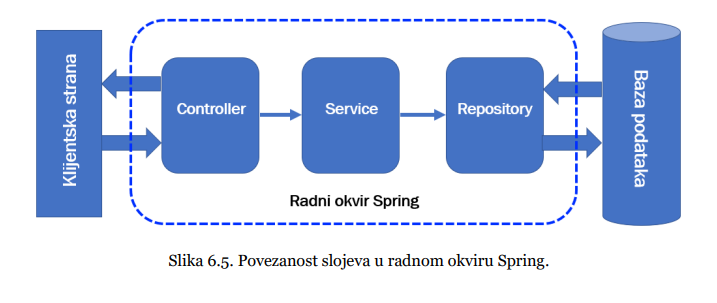
\includegraphics[scale=0.8]{slike/viseslojna_arhitekt.PNG} %veličina slike u odnosu na originalnu datoteku i pozicija slike
			\centering
			\caption{Primjer višeslojne arhitekture korištenjem radnog okvira Spring}
			\label{fig:arhitektura}
		\end{figure}

	
		

		

				
		\section{Baza podataka}
			
			\textbf{\textit{dio 1. revizije}}\\
			
		Za potrebe sustava koristit će se relacijska baza podataka koja nam omogućuje jednostavnije modeliranje stvarnog svijeta. Baza je implementirana u PostgreSQL-u zbog njegove jednostavnosti i jer je tim najbolje upoznat s tim sustavom; njegovim limitacijama i pravilima. Entiteti stvarnog svijeta su prevedeni kao tablice (relacije) koje imaju ime i svoj skup atributa. Baza podataka osigurava nam jednostavnu pohranu, umetanje, izmjenu i dohvat podataka, te garantira njihovu sigurnost. Baza podataka koristi sljedeće atribute:
		\begin{packed_item}
		\setlength\itemindent{24pt}
		\item prijave
		\item lokacije
		\item slike
		\item sorisnici
		\item tipovi{\_}ostecenja
		\item gradski{\_}uredi
		\end{packed_item}
		
		
			\subsection{Opis tablica}
			

				\textbf{prijave} je entitet koji sadrži sve važne informacije o podnesenim prijavama. Sastoji se od atributa:id, ostecenje{\_}id, lokacija{\_}id, kreator{\_}id, parent{\_}prijava{\_}id, prvo{\_}vrijeme{\_}prijave,
vrijeme{\_}otklona, naziv, opis. Ovaj entitet u vezi je One-to-One s tablicom lokacije preko atributa lokacija{\_}id, sa entitetom slike je u vezi One-to-Many preko atributa id. Sa entitetom tipovi{\_}ostecenja je u vezi One-to-Many preko atributa ostecenje{\_}id, u vezi Many-to-One sa entitetom korisnici preko atributa kreator{\_}id, te je sama sa sobom u refleksivnoj vezi One-to-Many preko atributa id.\\
				
				
				\begin{longtblr}[
					label=none,
					entry=none
					]{
						width = \textwidth,
						colspec={|X[6,l]|X[6, l]|X[20, l]|}, 
						rowhead = 1,
					} %definicija širine tablice, širine stupaca, poravnanje i broja redaka naslova tablice
					\hline \SetCell[c=3]{c}{\textbf{prijave}}	 \\ \hline[3pt]
					\SetCell{LightGreen}id & INT & jedinstveni identifikator prijave  	\\ \hline
					\SetCell{LightBlue}ostecenje{\_}id	& INT & jedinstveni identifikator tipa ostecenja   	\\ \hline 
					\SetCell{LightBlue}kreator{\_}id & INT &  jedinstvani identifikator korisnika koji je poslao prijavu \\ \hline 
					\SetCell{LightBlue}parent{\_} prijava{\_}id & INT & jedinstveni identifikator prijave na koju se prijava nadovezala		\\ \hline 
					 prvo{\_}vrijeme\_ prijave	& INT &  vrijeme slanja prijave 	\\ \hline
					 vrijeme{\_}otklona	& INT &  vrijeme otklona prijave 	\\ \hline 
					 opis & VARCHAR &  opis poslane prijave 	\\ \hline
					 naziv	& INT &  konkretno ime poslane prijave 	\\ \hline
					\end{longtblr}
					
					\textbf{lokacije} je entitet koji sadrži osnovne podatke o geografskoj lokaciji pojedine prijave. Sastoji se od atributa: lokacija{\_}id, latitude, longitude. Preko atributa id je povezana vezom One-to-One sa relacijom Prijave.\\
				
				\begin{longtblr}[
					label=none,
					entry=none
					]{
						width = \textwidth,
						colspec={|X[6,l]|X[6, l]|X[20, l]|}, 
						rowhead = 1,
					} %definicija širine tablice, širine stupaca, poravnanje i broja redaka naslova tablice
					\hline \SetCell[c=3]{c}{\textbf{Lokacije}}	 \\ \hline[3pt]
					\SetCell{LightGreen}lokacija{\_}id & INT &  	jedinstveni identifikator prijave 	\\ \hline
					latitude & INT & geografska latituda lokacije   	\\ \hline 
					longitude & INT & geografska longituda lokacije   	\\ \hline 
				\end{longtblr}
				
				\textbf{korisnici} je entitet koji sadrži osobne podatke o registriranim korisnicima kao i njihovu pripadnost vijecu i ulogu koju obnašaju u sustavu. Sastoji se od atributa: id, ime, prezime, username, email, password, ured{\_}id, role, active. Povezani su sa relacijom prijave u vezi One-to-Many preko atributa id, te sa relacijom gradski{\_}uredi u vezi Many-to-One preko atributa ured{\_}id.\\
				
				\begin{longtblr}[
					label=none,
					entry=none
					]{
						width = \textwidth,
						colspec={|X[6,l]|X[6, l]|X[20, l]|}, 
						rowhead = 1,
					} %definicija širine tablice, širine stupaca, poravnanje i broja redaka naslova tablice
					\hline \SetCell[c=3]{c}{\textbf{korisnici}}	 \\ \hline[3pt]
					\SetCell{LightGreen}id & INT & jedinstveni identifikator korisnika  	\\ \hline
					ime	& VARCHAR & ime registriranog korisnika   	\\ \hline
					prezime	& VARCHAR & prezime registriranog korisnika   	\\ \hline
					username	& VARCHAR & korisničko ime registriranog korisnika   	\\ \hline 
					email & VARCHAR & e-mail adresa registriranog korisnika   	\\ \hline
					password  & VARCHAR & lozinka za prijavu registriranog korisnika   	\\ \hline
					\SetCell{LightBlue}ured{\_}id & INT &  jedinstvani identifikator vijeca/ureda kojem pripada \\ \hline 
					active & INT & jedinstveni token sesije prijave korisnika		\\ \hline 
					 role & VARCHAR &  uloga koju korisnik obnaša u sustavu 	\\ \hline 
				\end{longtblr}
				
				\textbf{slike} je entitet koji sadrži podatke vezane za sliku podnešene prijave. Sastoji se od atributa: id, podatak, prijava{\_}id. Preko entiteta prijava{\_}id je povezan tablicom prijave u vezi Many-to-One.\\
				
				\begin{longtblr}[
					label=none,
					entry=none
					]{
						width = \textwidth,
						colspec={|X[6,l]|X[6, l]|X[20, l]|}, 
						rowhead = 1,
					} %definicija širine tablice, širine stupaca, poravnanje i broja redaka naslova tablice
					\hline \SetCell[c=3]{c}{\textbf{slike}}	 \\ \hline[3pt]
					\SetCell{LightGreen}id & INT &  	jedinstveni identifikator slike pojedine prijave	\\ \hline
					podatak & VARCHAR & string bitova koji sadrže sliku   	\\ \hline 
					\SetCell{LightBlue}prijava{\_}id & INT & jedinstveni identifikator prijave za koju je poslana slika   	\\ \hline 
				\end{longtblr}
				
				\textbf{tipovi{\_}osetecenja} je entitet koji sadrži podatke vezane za opis oštećenja kao i id ureda koji se bavi tim tipom oštećenja. Sastoji se od atributa: id, naziv. Preko atributa id je povezan sa relacijom prijave u vezi Many-to-One, te je sa relacijom gradski{\_}uredi u vezi One-to-One povezan preko istog atributa id.\\
				
				\begin{longtblr}[
					label=none,
					entry=none
					]{
						width = \textwidth,
						colspec={|X[6,l]|X[6, l]|X[20, l]|}, 
						rowhead = 1,
					} %definicija širine tablice, širine stupaca, poravnanje i broja redaka naslova tablice
					\hline \SetCell[c=3]{c}{\textbf{tipovi\_ ostecenja}}	 \\ \hline[3pt]
					\SetCell{LightGreen}id & INT &  	jedinstveni identifikator vrste oštećenja	\\ \hline
					naziv & VARCHAR & naziv konkretnog oštećenja   	\\ \hline  
				\end{longtblr}
				
				\textbf{gradski{\_}uredi} je entitet koji sadrži podatke vezane za opis pojedinog vijeca/ureda koji je zadužen za otklanjanje određenog tipa oštećenja. Sastoji se od atributa: id, naziv i ostecenje{\_}id. Preko atributa ostecenje{\_}id je povezan sa relacijom tipovi{\_}ostecenja u vezi Many-to-One, te je povezan sa relacijom korisnici preko atributa id u vezi One-to-Many.\\
				
				\begin{longtblr}[
					label=none,
					entry=none
					]{
						width = \textwidth,
						colspec={|X[6,l]|X[6, l]|X[20, l]|}, 
						rowhead = 1,
					} %definicija širine tablice, širine stupaca, poravnanje i broja redaka naslova tablice
					\hline \SetCell[c=3]{c}{\textbf{gradski{\_}uredi}}	 \\ \hline[3pt]
					\SetCell{LightGreen}id & INT &  jedinstveni identifikator pojedinog registriranog vijeća/ureda	\\ \hline
					naziv & VARCHAR & puni naziv vijćea u aplikaciji\\ \hline 
					\SetCell{LightBlue}ostecenje{\_}id & INT & identifikator vrste oštećenja koje za koje je taj ured zadužen\\ \hline
				\end{longtblr}
				
				
			
			\subsection{Dijagram baze podataka}
				\begin{figure}[H]
			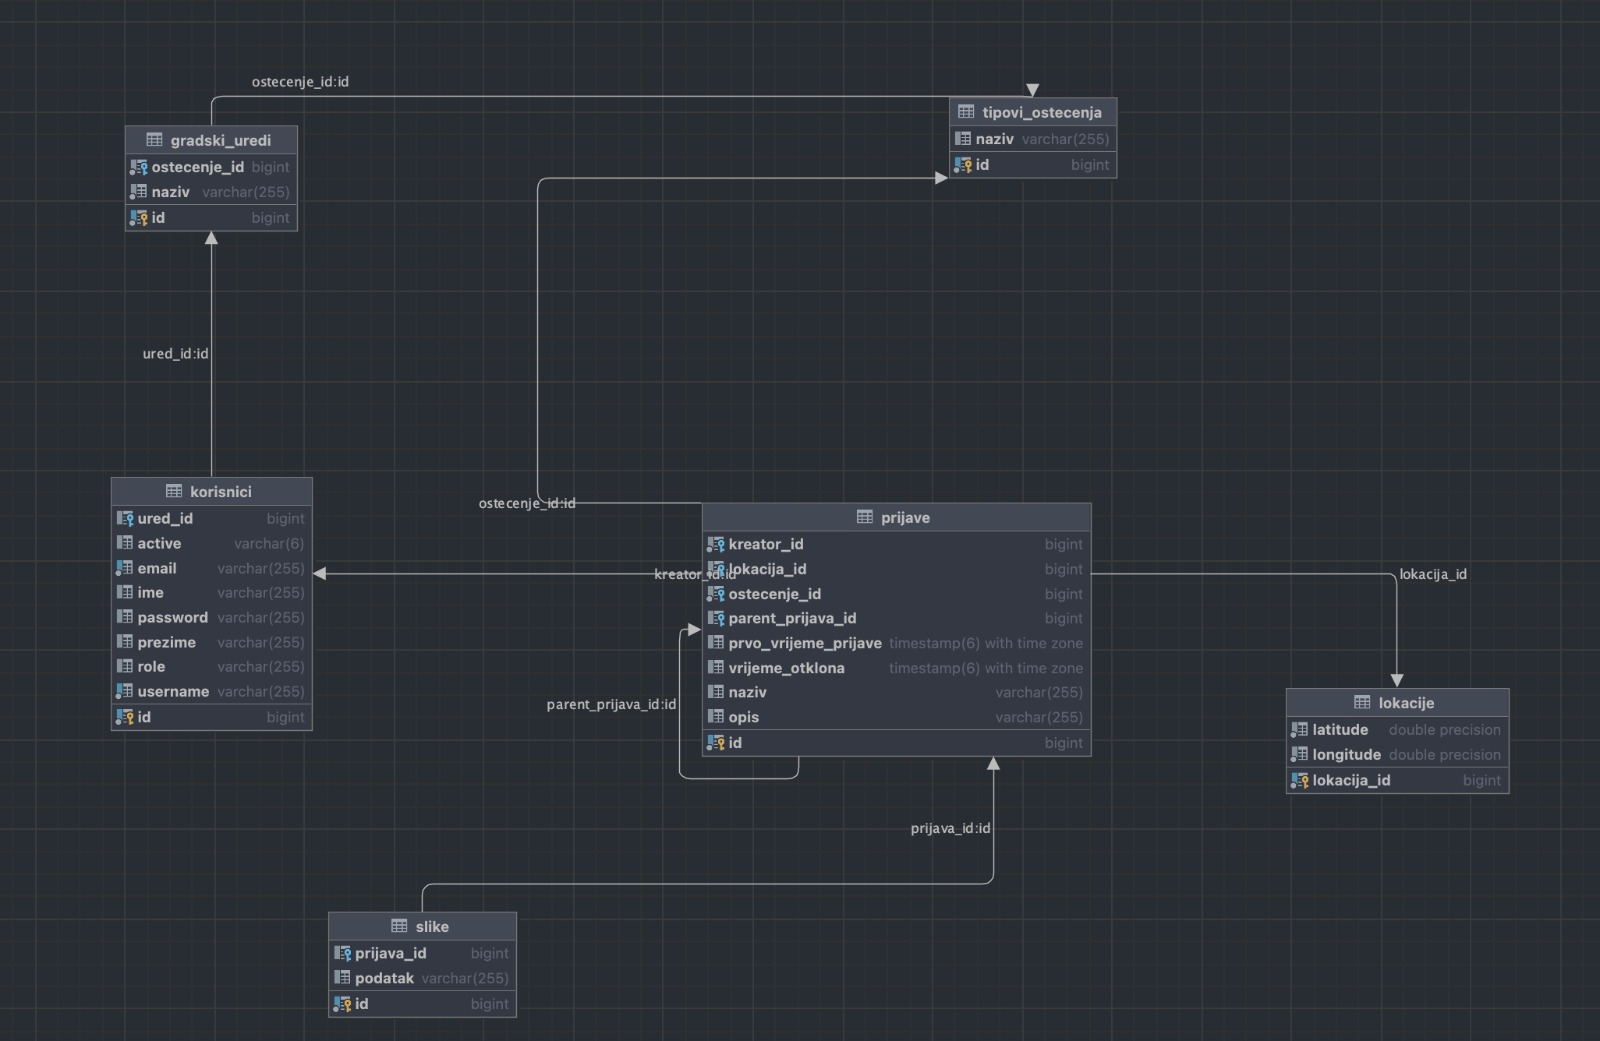
\includegraphics[scale=0.3]{slike/erBaza.PNG} %veličina slike u odnosu na originalnu datoteku i pozicija slike
			\centering
			\caption{Relacijski dijagram baze podataka}
			\label{fig:bazapod}
		\end{figure}
			
			\eject
			
			
		\section{Dijagram razreda}
		
			Na slikama 4.3 i 4.4 prikazani su razredi i njihove relacije na serverskoj strani aplikacije. Konkretnije rečeno prikazani su modeli i kontroleri. \\
			
			Svi kontroleri nasljeđuju razred Controller. Metode koje su u njima implementirane ovise o DTO objektima, koji se realiziraju pomoću metoda implementiranih u Domain dijelu razreda.
			
			
				\begin{figure}[H]
			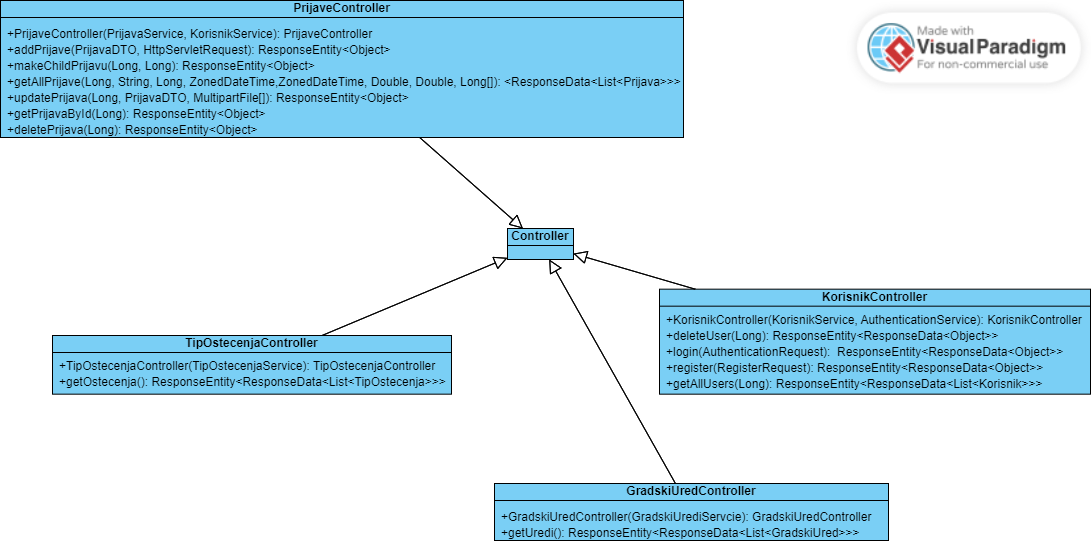
\includegraphics[scale=0.3]{slike/kontroleri.PNG} %veličina slike u odnosu na originalnu datoteku i pozicija slike
			\centering
			\caption{Dijagram razreda - Controllers dio}
			\label{fig:bazapod}
		\end{figure}
		
		\pagebreak
		
		Domain dio razreda preslikava strukturu baze podataka, te svi razredi nasljeđuju razred Model. Ovako ilustrirani razredi su zapravo odraz onih relacija koji su zapisani u bazi podataka, te direktno komunciraju sa bazom podataka. Razred Korisnik je ilustracija bilo kojeg registriranog usera koji ima svoju ulogu (povezan sa enumom Role), te može podnijeti prijavu u sustav (pvezanost sa razredom Prijava preko private atributa prijave). Prijave kada se konstruiraju zadaje im se lokacija (pa su preko atributa lokacija povezane sa razredom Lokacija), slika (agregatna povezanost sa razredom Slika preko varijable slike) i tip ostecenja (agregatna povezanost sa razredom tipOstecenja preko atributa tipOstecenja). Razred GradskiUred je reprezentacija gradskig ureda koje je povezan sa tipom oštećenja preko atributa tipOstecenja. \\
		
		
			\begin{figure}[H]
			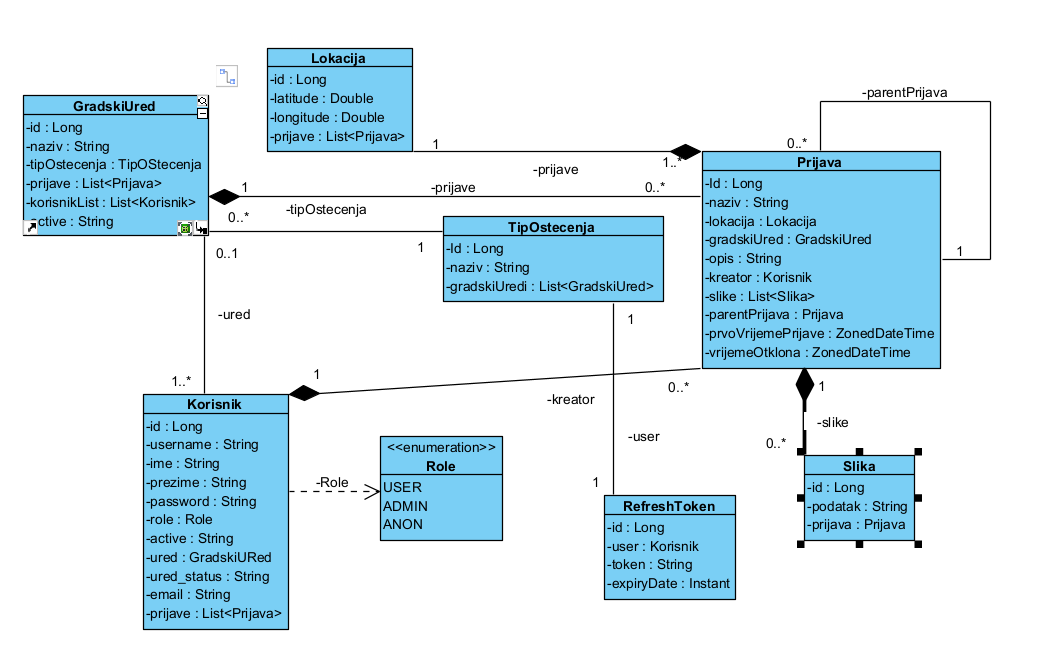
\includegraphics[scale=0.3]{slike/domain.PNG} %veličina slike u odnosu na originalnu datoteku i pozicija slike
			\centering
			\caption{Dijagram razreda - Controllers dio}
			\label{fig:bazapod}
		\end{figure}
			
			
			\eject
		\section{Dijagram stanja}
			
			
			\textbf{\textit{dio 2. revizije}}\\
			
			\textit{Potrebno je priložiti dijagram stanja i opisati ga. Dovoljan je jedan dijagram stanja koji prikazuje \textbf{značajan dio funkcionalnosti} sustava. Na primjer, stanja korisničkog sučelja i tijek korištenja neke ključne funkcionalnosti jesu značajan dio sustava, a registracija i prijava nisu. }
			
			
			\eject 
		
		\section{Dijagram aktivnosti}
			
			\textbf{\textit{dio 2. revizije}}\\
			
			 \textit{Potrebno je priložiti dijagram aktivnosti s pripadajućim opisom. Dijagram aktivnosti treba prikazivati značajan dio sustava.}
			
			\eject
		\section{Dijagram komponenti}
		
			\textbf{\textit{dio 2. revizije}}\\
		
			 \textit{Potrebno je priložiti dijagram komponenti s pripadajućim opisom. Dijagram komponenti treba prikazivati strukturu cijele aplikacije.}
	\chapter{Implementacija i korisničko sučelje}
		
		
		\section{Korištene tehnologije i alati}
		
			Dio  zadužen za frontend i komunikaciju s korisnikom je ostvaren pomoću knjižnice \href{https://react.dev/}{React}, te je pisan u programskom jeziku
			\href{https:www.typescriptlang.org/}{TypeScript}. React, kao bibilioteka je široko raspostranjen u području stvaranja korisničkog sučelja. Jedna od glavnih prednosti jest objedinjavanje visokih performansi brzine aplikacije, korištenjem 
virtualnog DOM-a, te omogućuje podršku za ponovnu uporabivost komponenti i nadogradnju sustava (zbog svoje enkapsuliranosti). Razvila ga je grupa Meta (Facebook) i naglask se stavlja na njegovu pripadnost knjižnicama, a ne radnim okvirima. \\
			Razvojno okruženje u kojem je pisan cijeli frotend je \href{https://code.visualstudio.com/}{Visual Studio Code}(tzv. VSC). VSC je integrirano razvojno okuženje u vlasništvu tvrtke Microsoft. Danas je to jedna od najkorišenijih tehnologija za uređivanje i pisanje koda, a to je s dobrim razlogom jer on nudi mnoštva ekstenzija za razne programske jezike (pa tako i za TypeScript u kojem je naša aplikacija pisana), ali i jednostavne funkcionalnosti koje ispadaju uvelike korisne te olakšavaju posao pisanja koda, a neke od tih su: debugger, IntelliSense koji služi kao autofill i ugrađena podrška za Git. \\
			Backend sustava pisan je u programskom jeziku \href{https://www.java.com/en/}{Java} korištenjem radnog okvira \href{https://spring.io/projects/spring-boot/}{Spring Boot}. Spring Boot je implementiran kao specijalizacija generaliziranijeg radnog okvira Spring, a omogućuje izradu stand-alone aplikacija. Dobrim dijelom olakšava posao izgradnje sustava jer sam konfigurira funckionalnosti Springa, ali i sam ima već podešene one dijelove web aplikacije koji se učestalo koriste (npr. servleti).\\
			Cijeli backend je pisan u razvojnom okruženju \href{https://www.jetbrains.com/idea/}{InntelliJ IDEA}. To je integrirano razvojno sučelje u vlasništvu kompanije JetBrains, a prevladavajuće je u području pisanja porgrama u Javi i Kotlinu. Velike funkcionalnosti koje koristi su coding assistance, remote cooperation kao i jednostavnost uporabe. \\
			Za dokumentaciju se koristio programski jezik \href{https://www.latex-project.org//}{$LaTeX$}. $LaTeX$ je jezik za pisanje strukturiranih tesktova, piše se kao običan tekst sa dodanom semantičkom strukturom (ne prikazuje se kao konačan proizvod kao npr. Microsoft Word) što mu omogućuje stabilniji rad, a sve što zahtjeva je instalriana distribucija TeX-a; što je u našem slučaju \href{https://miktex.org/}{MiKTeX}. Dokumentacija je pisana u uređivaču teksta zvanom \href{https://www.xm1math.net/texmaker/}{Texmaker} koji se ističe po jednostavnosti pisanju $LaTeX$ dokumenata kao i u svojoj dostupnosti.\\
			Realizacija baze podataka izvedena je U \href{https://www.postgresql.org/}{PostgreSQL-u}. PostgreSQL je open-source sustav za upravljanje relacijama bazama podataka. Uvelike naglasak stavlja na ispunjavanju ACID svojstava pri izvođenju transakcija i pristupačan je za korištenje. Unutar PostgreSQL-a korišten je \href{https://www.pgadmin.org/}{pgAdmin} kao grafički alat za upravljanje bazama podataka i njihovh shema.
			U izradi UML dijagrama korištene su dvije tehnologije: \href{https://astah.net/}{Astah} i \href{https://www.visual-paradigm.com/}{Visual Paradigm}. Oba se alata ističu po svojoj rasprostranjenosti tako što omogućavaju izbor kreiranja svakojakih dijagrama, ali i po svojoj jednostavnosti. Razlika je u tome što je Astah porgram koje se pokreće lokalno na računalu, a Visual Paradigm se pokreće online i sprema trenutne izmjene po izboru lokalno ili na Cloud.\\
			Kako bi se lakše upravljalo verzijama projekta, korišten je \href{https://git-scm.com/}{Git}. Git je besplatan, open source sustav koji se koristi za upravljanje kako manjih, tako i većih projekata. Prednosti su mu brzina, jednostavnost i lakoća upravljanja projektima u timskom radu. Vanjski repozitorij projekta se nalazi na besplatnoj web platformi \href{https://github.com/}{GitHub} koja omogućuje lako upravljanje projektom svim sudionicima repozitorija. \\
			Za produkciju aplikacije korišen je cloud sustav \href{https://render.com/}{Render}. Render olakšava puštanje aplikacija u pogon kako bi bile javno dostupne za pronalazak an internetu. \\
			Kako bi se u timu maksimalno olakšala komunikacija članova kroišen je \href{https://discord.com/}{Discord}. Discord je društvena platforma u kojoj je naglasak na jednostavnosti postizanja glasovne, video i tekstne komunikacije u zajednicama koje se nazivaju serveri kojima se pristupa pomoću poveznice, a omogućuju kavlitetan integritet tima (zajednice).
			\eject 
		
	
		\section{Ispitivanje programskog rješenja}
	
			
			\subsection{Ispitivanje komponenti}
			\textit{Potrebno je provesti ispitivanje jedinica (engl. unit testing) nad razredima koji implementiraju temeljne funkcionalnosti. Razraditi \textbf{minimalno 6 ispitnih slučajeva} u kojima će se ispitati redovni slučajevi, rubni uvjeti te izazivanje pogreške (engl. exception throwing). Poželjno je stvoriti i ispitni slučaj koji koristi funkcionalnosti koje nisu implementirane. Potrebno je priložiti izvorni kôd svih ispitnih slučajeva te prikaz rezultata izvođenja ispita u razvojnom okruženju (prolaz/pad ispita). }
			
			U ovom potpoglavlju razrađeno je testiranje backend dijela aplikacije sa konkretno implementiranim testovima. Testovi su JUnit testovi, a na slici 5.1 prikazan je vremenski interval svakog od 7 testova, kao i verifikacija za njihov prolaz.\\
			\\
			\textbf{Test 1: Metoda koja vraća registrirani gradski ured u bazi podataka}\\
			\\ U ovom je testu cilj bio iz baze podataka "izvući" jedan gradski ured koji odgovara određenim atributima. Dobivena relacije je perotvorena u DTO oblik za lakše rukovanje u sustavu.\\
			\begin{figure}[H]
			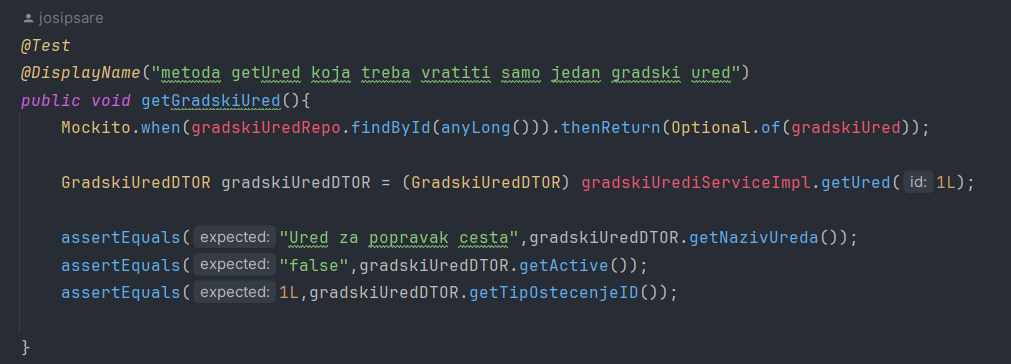
\includegraphics[scale=0.4]{slike/getUred.PNG} %veličina slike u odnosu na originalnu datoteku i pozicija slike
			\centering
			\caption{Pregled gradskog ureda određenih atributa metodom getGradskiUred()}
			\label{fig:implementacija}
		\end{figure}
			
			
			 \textbf{Test 2: Metoda koja provjerava postojanost novostvorenog ureda}\\
			\\ U ovom je testu cilj bio pregledati sadržaj baze podataka nakon stvaranja novog gradskog ureda, kokretnije ispravnost zapisa njegovih atributa.
			
			\begin{figure}[H]
			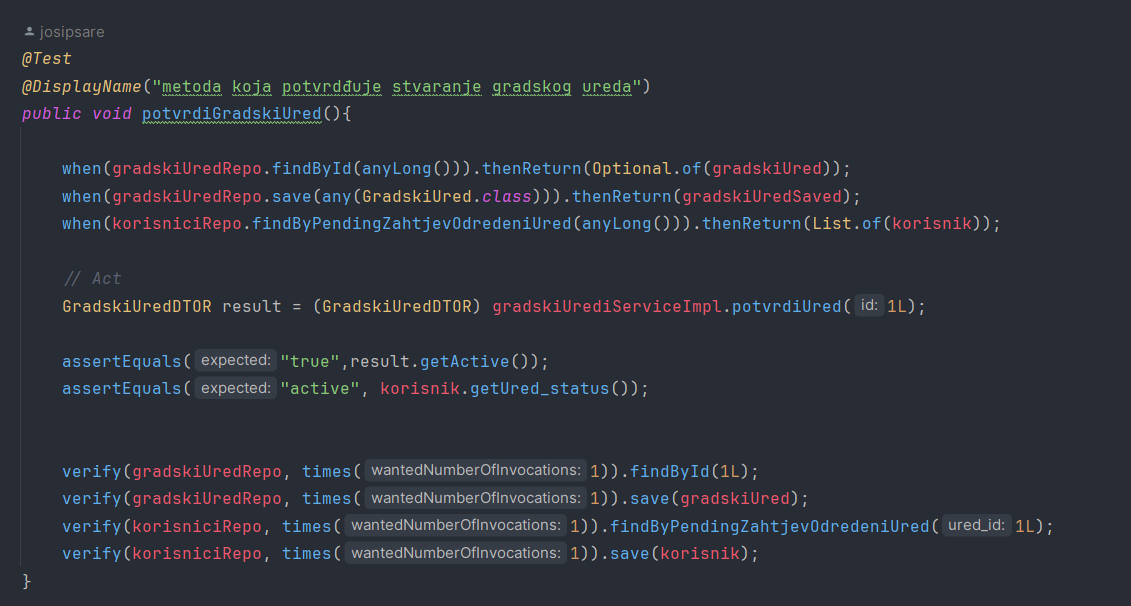
\includegraphics[scale=0.4]{slike/potvrdiUred.PNG} %veličina slike u odnosu na originalnu datoteku i pozicija slike
			\centering
			\caption{Potvrđivanje novonastalog gradskog ureda metodom potvrdiGradskiUred()}
			\label{fig:implementacija}
		\end{figure}
		
		
		\textbf{Test 3: Pretraživanje nepostojećeg korisnika u bazi podataka}\\
			\\ U ovom je testu cilj bio pronaći nepostojećeg korisnika u bazi podataka i uočiti baca li se adekvatna iznimka.
			
			\begin{figure}[H]
			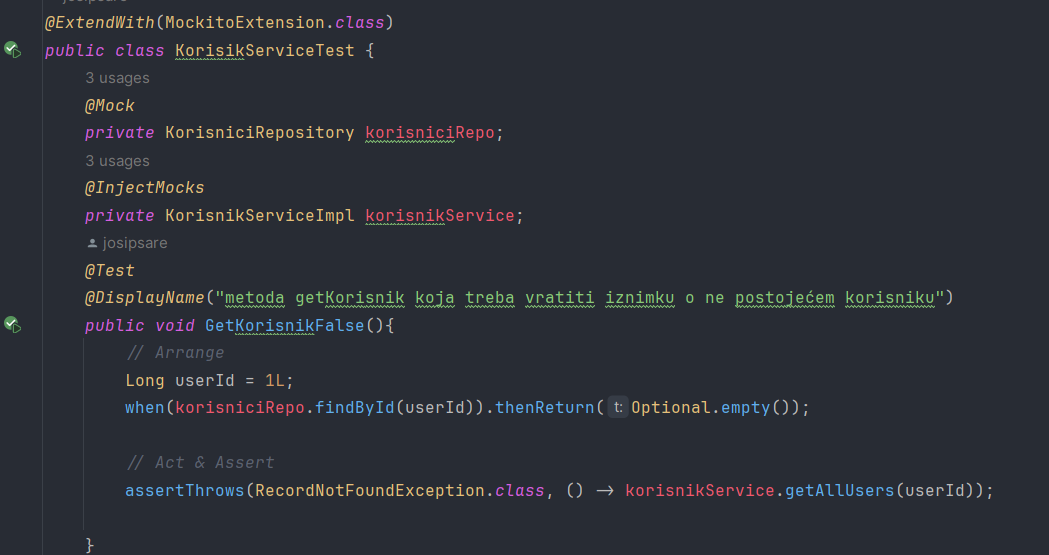
\includegraphics[scale=0.6]{slike/nepostojeciUser.PNG} %veličina slike u odnosu na originalnu datoteku i pozicija slike
			\centering
			\caption{Pregled postojanosti nepostojećeg korisnika}
			\label{fig:implementacija}
		\end{figure}
		
		\pagebreak 
		
		\textbf{Test 4: Pregled svih postojećih korisnika u sustavu}\\
			\\ U testu prikazanom na idućoj slici kreirano više korisnika sa vlastitim atributima. Novonastali korisnici su dodani u listu te je na testa kraju vraćena odgovarajuća lista u koju su dodani spomenuti korisnici kako bi se provejrio zapis objekata u bazi podataka.
			
			\begin{figure}[H]
			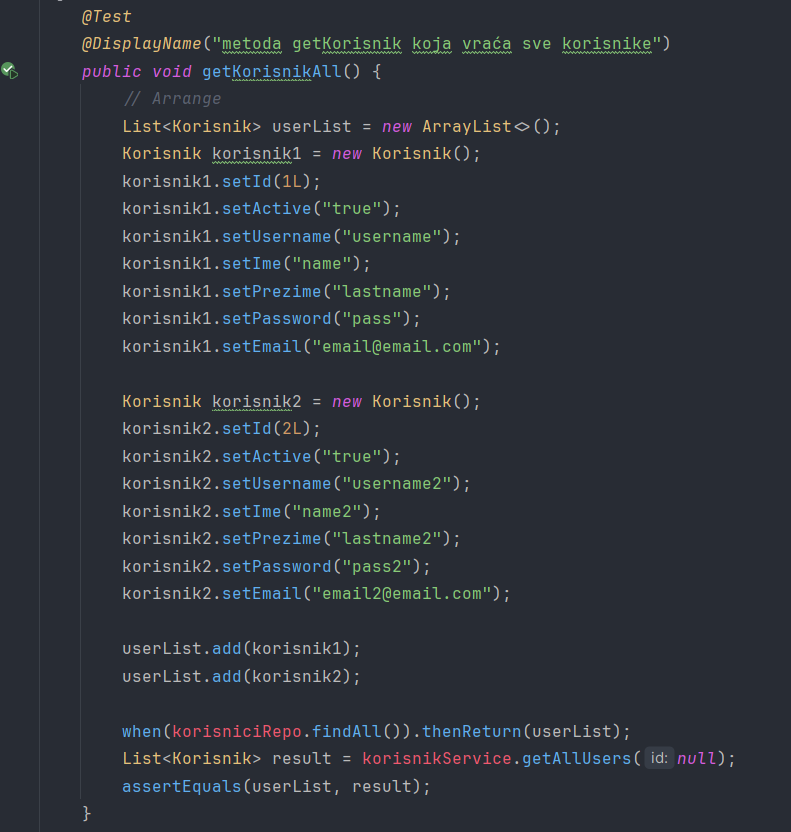
\includegraphics[scale=0.6]{slike/allUsers.PNG} %veličina slike u odnosu na originalnu datoteku i pozicija slike
			\centering
			\caption{Pregled liste svih postojećih korisnika sa svojim atrubutima u sustavu metodom getKorisnikAll()}
			\label{fig:implementacija}
		\end{figure}
		
		\textbf{Test 5: Registracija novog korinsika u sustav}\\
			\\ U testu broj pet kreiran je jedan user sa svojim pripadajućim atributima i spremljen u bazu podataka. Cilj je dobiti istog tog korisnika pretragom po određenom atributu i učiti ispravnost zapisa novonastalog objekta
			
			\begin{figure}[H]
			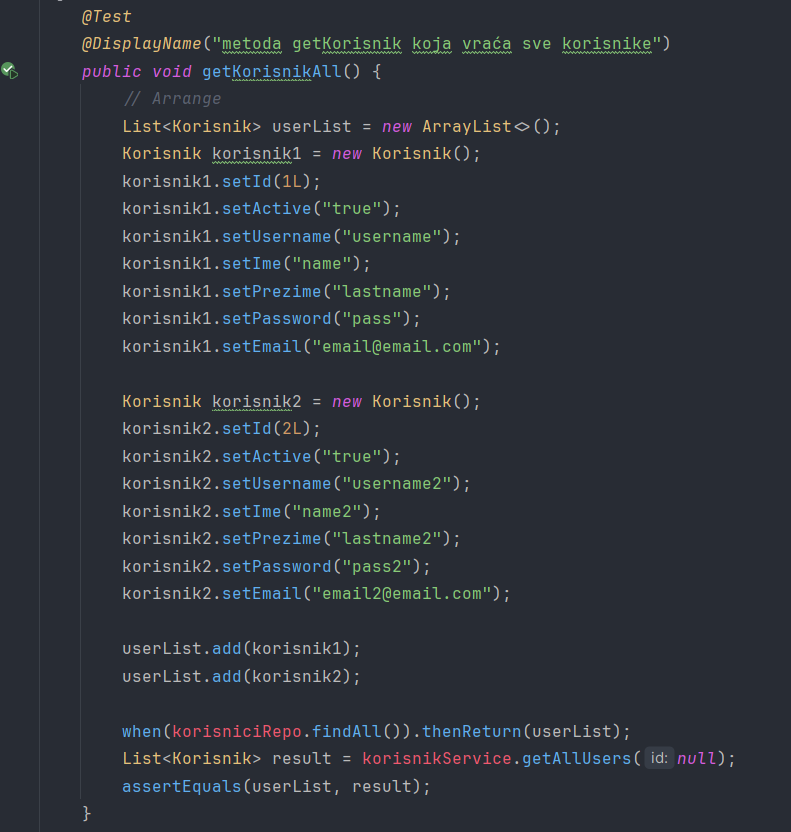
\includegraphics[scale=0.5]{slike/allUsers.PNG} %veličina slike u odnosu na originalnu datoteku i pozicija slike
			\centering
			\caption{Registracija novog korisnika}
			\label{fig:implementacija}
		\end{figure}
		
		\textbf{Test 6: Pregled svih prijava u sustavu}\\
			\\ U predzadnjem provedenom testu kreirane su nove prijave. Cilj je bio iz baze podataka izvući sve porstojeće prijave u sustavu kako bi se provjerila točnost njihovog zapisa u bazi podataka.
			
			\begin{figure}[H]
			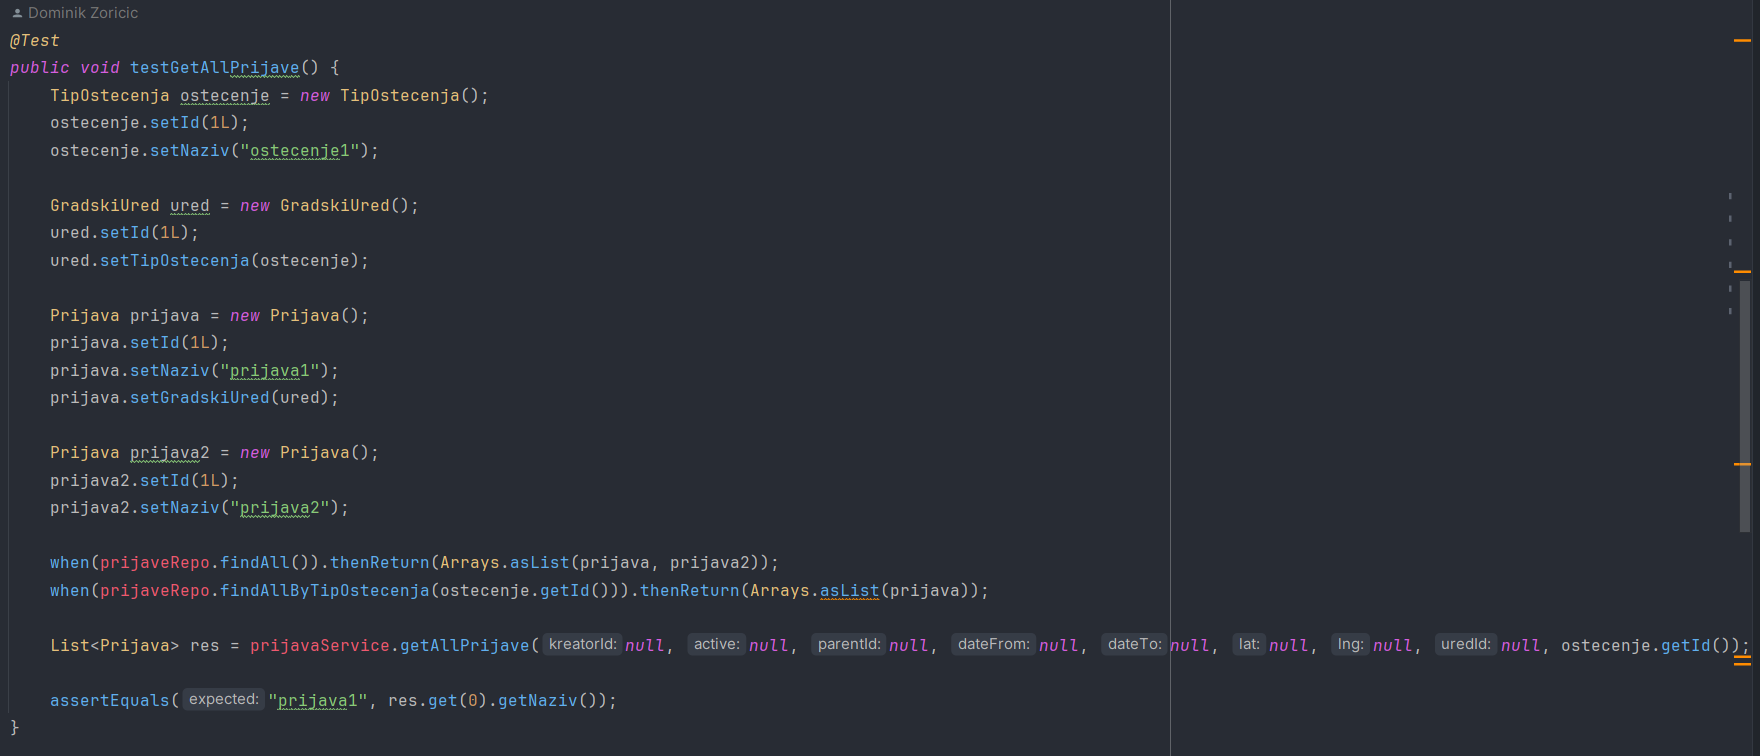
\includegraphics[scale=0.5]{slike/svePrijave.PNG} %veličina slike u odnosu na originalnu datoteku i pozicija slike
			\centering
			\caption{Pretraga svih prijava regsitriranih u bazi podataka}
			\label{fig:implementacija}
		\end{figure}
		
		\textbf{Test 7: Dodavanje nove prijave u sustav}\\
			\\ U zadnjem provedenom testu kreirane su nove prijave. Cilj je bio potvrditi postojanost zapisa nove prijave u bazi podataka.
			
			\begin{figure}[H]
			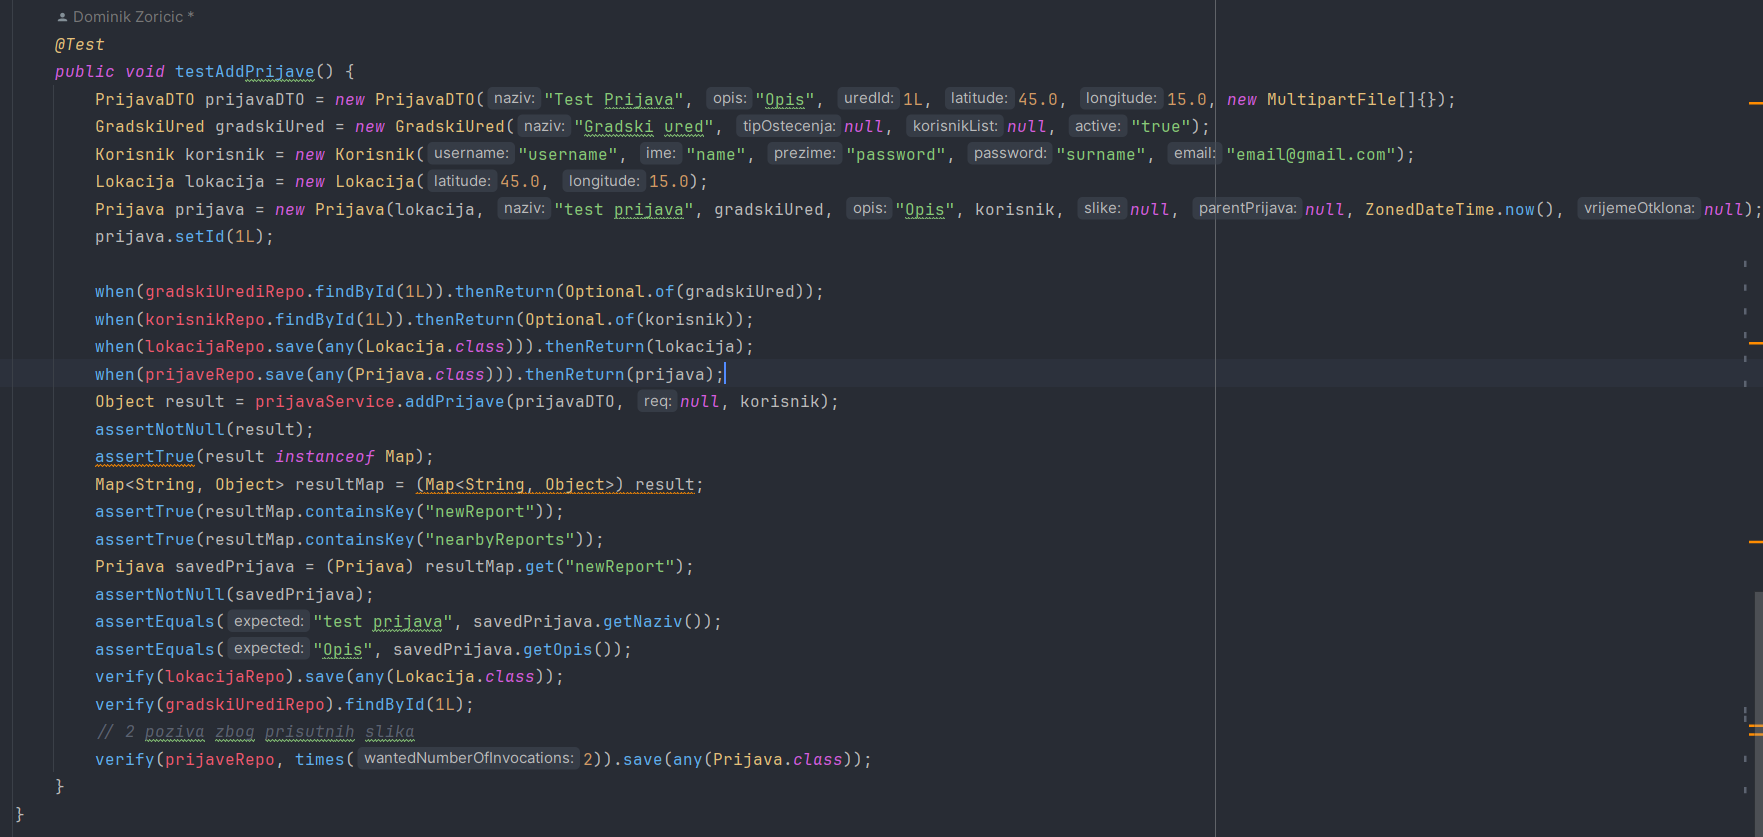
\includegraphics[scale=0.5]{slike/addPrijava.PNG} %veličina slike u odnosu na originalnu datoteku i pozicija slike
			\centering
			\caption{Kreacija novih prijava u sustavu}
			\label{fig:implementacija}
		\end{figure}
			
			
			
			\subsection{Ispitivanje sustava}
			
			 \textit{Potrebno je provesti i opisati ispitivanje sustava koristeći radni okvir Selenium\footnote{\url{https://www.seleniumhq.org/}}. Razraditi \textbf{minimalno 4 ispitna slučaja} u kojima će se ispitati redovni slučajevi, rubni uvjeti te poziv funkcionalnosti koja nije implementirana/izaziva pogrešku kako bi se vidjelo na koji način sustav reagira kada nešto nije u potpunosti ostvareno. Ispitni slučaj se treba sastojati od ulaza (npr. korisničko ime i lozinka), očekivanog izlaza ili rezultata, koraka ispitivanja i dobivenog izlaza ili rezultata.\\ }
			 
			 \textit{Izradu ispitnih slučajeva pomoću radnog okvira Selenium moguće je provesti pomoću jednog od sljedeća dva alata:}
			 \begin{itemize}
			 	\item \textit{dodatak za preglednik \textbf{Selenium IDE} - snimanje korisnikovih akcija radi automatskog ponavljanja ispita	}
			 	\item \textit{\textbf{Selenium WebDriver} - podrška za pisanje ispita u jezicima Java, C\#, PHP koristeći posebno programsko sučelje.}
			 \end{itemize}
		 	\textit{Detalji o korištenju alata Selenium bit će prikazani na posebnom predavanju tijekom semestra.}
			
			\eject 
		
		
		\section{Dijagram razmještaja}
			
			 Dijagram razmještaja opisuje topologiju virtualnih i fizičkih čvorova i komunikacijske puteve između istih. U našem slučaju sustav je temeljen na klijent-poslužitelj odnosu u kojem klijentsko računalo http protokolom razmjenjuje podatke sa serverskim uređajem. Serverska je strana implemenirana pomoću web servisa Render.
			 
			 \begin{figure}[H]
			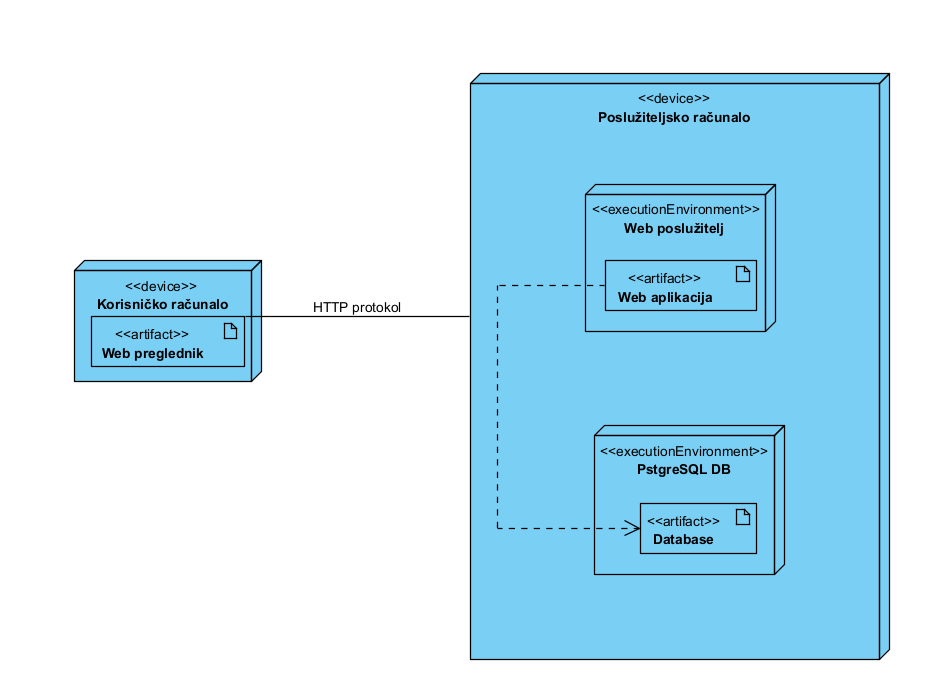
\includegraphics[scale=0.5]{slike/deploymentDiagram.PNG} %veličina slike u odnosu na originalnu datoteku i pozicija slike
			\centering
			\caption{Dijagram razmještaja}
			\label{fig:implementacija}
		\end{figure}
			
			\eject 
		
		\section{Upute za puštanje u pogon}
		
			\subsection{Konfiguracija frontenda}
			Pri konfiguraciji frontenda na poslužitelju Render potrebno je GitHub račun spojiti s Renderom. Idući je korak kreirati novi servis i odabrati projekt Gradska šteta. Regija je Frankfurt (EU Central), za root directory se odabire frontend. Environment se treba postaviti na Node, dok je build command potrebno postaviti na npm run build, a start command na npm run server. Zadnji korak je postaviti evnironment varijable ka na idućoj slici i kliknuti Create Web Server.
			
			
			\begin{figure}[H]
			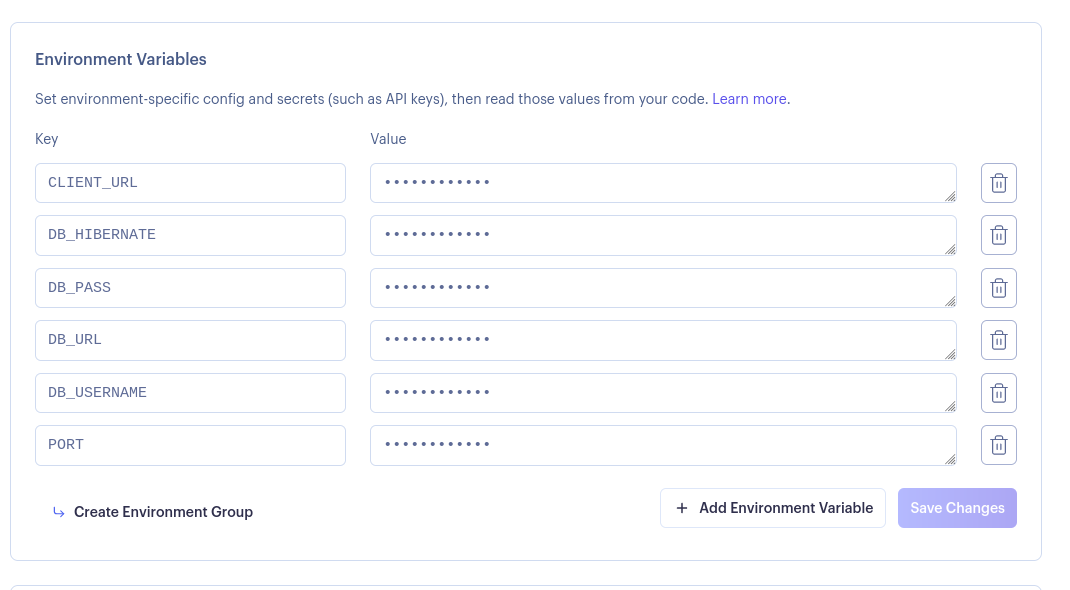
\includegraphics[scale=0.4]{slike/frontendEnvironment.PNG} %veličina slike u odnosu na originalnu datoteku i pozicija slike
			\centering
			\caption{Environment varijable za frontend dio}
			\label{fig:implementacija}
		\end{figure}
		
		\subsection{Konfiguracija backenda}
			
			Pri konfiguraciji backenda na poslužitelju Render potrebno je GitHub račun spojiti s Renderom. Idući je korak kreirati novi servis i odabrati projekt Gradska šteta. Kao regiju treba odabrati Frankfurt (EU Central), za root directory se odabire backend. Dockerfile se nalazi u backend direktoriju (/backend), a Docker Build Context directory je /backend. Na idućoj slici su prikazane environment varijable koje treba postaviti i kliknuti na Create Web Server.
			
			\begin{figure}[H]
			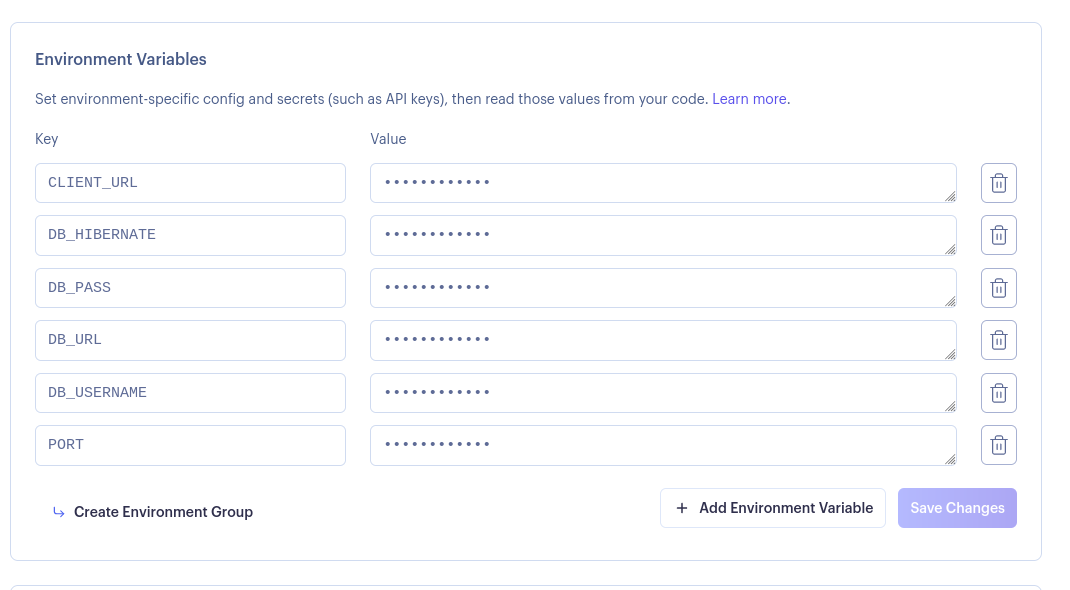
\includegraphics[scale=0.4]{slike/backendEnvironment.PNG} %veličina slike u odnosu na originalnu datoteku i pozicija slike
			\centering
			\caption{Environment varijable za backend dio}
			\label{fig:implementacija}
		\end{figure}
		
		\subsection{Konfiguracija baze podataka}
			
			Pri konfiguraciji poslužitelja baze podataka na Renderu potrebno je postaviti ime baze zajedno sa imenom korisnika baze. Kao regiju postavizi Frankfurt(EU Central) i dovršiti kreiranje sa klikom na Create Database. Environment varijable prikazane su na slici \ref{fig:implementacijaBaze}.
			
			\begin{figure}[H]
			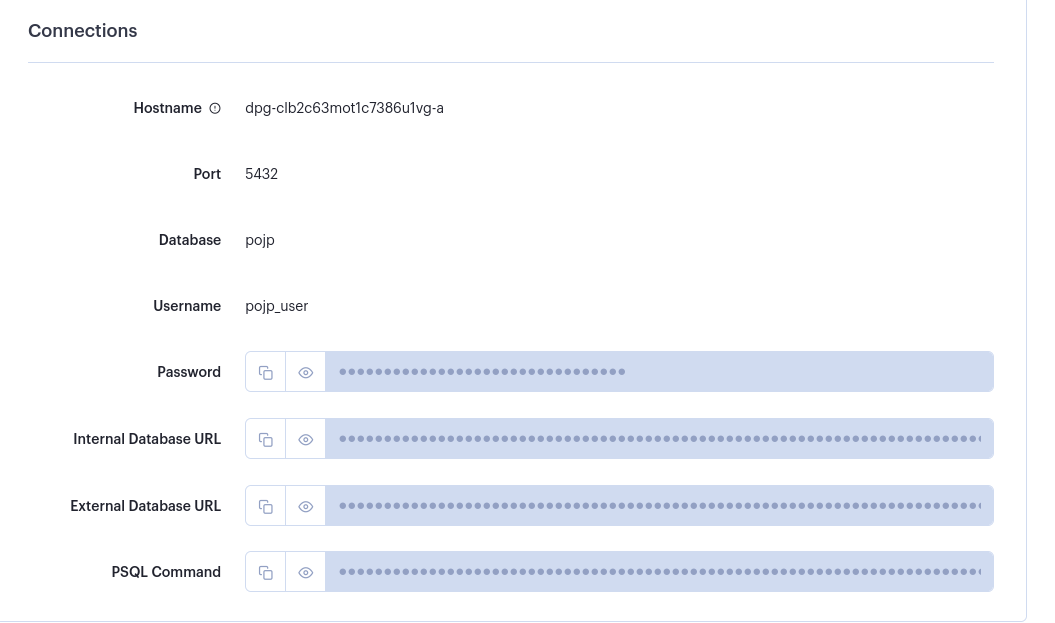
\includegraphics[scale=0.4]{slike/bazaEnvironment.PNG} %veličina slike u odnosu na originalnu datoteku i pozicija slike
			\centering
			\caption{Environment varijable za bazu podataka}
			\label{fig:implementacijaBaze}
		\end{figure}
			
			\eject 
	\chapter{Zaključak i budući rad}
		
		\textbf{\textit{dio 2. revizije}}\\
		
		 \textit{U ovom poglavlju potrebno je napisati osvrt na vrijeme izrade projektnog zadatka, koji su tehnički izazovi prepoznati, jesu li riješeni ili kako bi mogli biti riješeni, koja su znanja stečena pri izradi projekta, koja bi znanja bila posebno potrebna za brže i kvalitetnije ostvarenje projekta i koje bi bile perspektive za nastavak rada u projektnoj grupi.}
		
		 \textit{Potrebno je točno popisati funkcionalnosti koje nisu implementirane u ostvarenoj aplikaciji.}
		
		\eject 
	\chapter*{Popis literature}
		\addcontentsline{toc}{chapter}{Popis literature}
	 	
 		\textbf{\textit{Kontinuirano osvježavanje}}
	
		\textit{Popisati sve reference i literaturu koja je pomogla pri ostvarivanju projekta.}
		
		
		\begin{enumerate}
			
			
			\item  Programsko inženjerstvo, FER ZEMRIS, \url{http://www.fer.hr/predmet/proinz}
			
			\item  I. Sommerville, "Software engineering", 8th ed, Addison Wesley, 2007.
			
			\item  T.C.Lethbridge, R.Langaniere, "Object-Oriented Software Engineering", 2nd ed. McGraw-Hill, 2005.
			
			\item  The Unified Modeling Language, \url{https://www.uml-diagrams.org/}
			
			\item  Astah Community, \url{http://astah.net/editions/uml-new}
			
			\item  Visual Paradigm, \url{https://www.visual-paradigm.com/}
			
			\item  Wikipedia, \url{https://www.wikipedia.org/}
		\end{enumerate}
		
		 
	
	
	\begingroup
	\renewcommand*\listfigurename{Indeks slika i dijagrama}
	%\renewcommand*\listtablename{Indeks tablica}
	%\let\clearpage\relax
	\listoffigures
	%\vspace{10mm}
	%\listoftables
	\endgroup
	\addcontentsline{toc}{chapter}{Indeks slika i dijagrama}


	
	\eject 
		
	\chapter*{Dodatak: Prikaz aktivnosti grupe}
		\addcontentsline{toc}{chapter}{Dodatak: Prikaz aktivnosti grupe}
		
		\section*{Dnevnik sastajanja}
		
		\textbf{\textit{Kontinuirano osvježavanje}}\\
		
		 \textit{U ovom dijelu potrebno je redovito osvježavati dnevnik sastajanja prema predlošku.}
		
		\begin{packed_enum}
			\item  sastanak
			
			\item[] \begin{packed_item}
				\item Datum: 23. listopada 2023.
				\item Prisustvovali: Nikola Botić, 
				Nino Ćurko, Ivan Elez,
				Davor Najev, Josip Šare,
				Ivan Šimunić, Dominik Zoričić
				\item Teme sastanka:
				\begin{packed_item}
					\item  raspodjela uloga po članovima
					\item  odabir izvedbenih tehnologija
				\end{packed_item}
			\end{packed_item}
			
			\item  sastanak
			\item[] \begin{packed_item}
				\item Datum: 26. listopada 2023.
				\item Prisustvovali: Nikola Botić, 
				Nino Ćurko, Ivan Elez,
				Davor Najev, Josip Šare,
				Dominik Zoričić
				\item Teme sastanka:
				\begin{packed_item}
					\item  TODO
				\end{packed_item}
			\end{packed_item}

			\item  sastanak
			\item[] \begin{packed_item}
				\item Datum: u ovom formatu: \today
				\item Prisustvovali: I.Prezime, I.Prezime
				\item Teme sastanka:
				\begin{packed_item}
					\item  opis prve teme
					\item  opis druge teme
				\end{packed_item}
			\end{packed_item}
			
			%
			
		\end{packed_enum}
		
		\eject
		\section*{Tablica aktivnosti}
		
			\textbf{\textit{Kontinuirano osvježavanje}}\\
			
			 \textit{Napomena: Doprinose u aktivnostima treba navesti u satima po članovima grupe po aktivnosti.}

			\begin{longtblr}[
					label=none,
				]{
					vlines,hlines,
					width = \textwidth,
					colspec={X[7, l]X[1, c]X[1, c]X[1, c]X[1, c]X[1, c]X[1, c]X[1, c]}, 
					vline{1} = {1}{text=\clap{}},
					hline{1} = {1}{text=\clap{}},
					rowhead = 1,
				} 
			
				\SetCell[c=1]{c}{} & \SetCell[c=1]{c}{\rotatebox{90}{\textbf{Ivan Šimunić }}} & \SetCell[c=1]{c}{\rotatebox{90}{\textbf{Nino Ćurko }}} &	\SetCell[c=1]{c}{\rotatebox{90}{\textbf{Davor Najev }}} & \SetCell[c=1]{c}{\rotatebox{90}{\textbf{Nikola Botić }}} &	\SetCell[c=1]{c}{\rotatebox{90}{\textbf{Dominik Zoričić }}} & \SetCell[c=1]{c}{\rotatebox{90}{\textbf{Josip Šare }}} &	\SetCell[c=1]{c}{\rotatebox{90}{\textbf{Ivan Elez }}} \\  
				Upravljanje projektom 		& 1 & 2 & 2 & 2 & 2 & 2 & 2\\ 
				Opis projektnog zadatka 	&  &  &  &  &  &  & \\ 
				
				Funkcionalni zahtjevi       &  &  &  &  &  &  &  \\ 
				Opis pojedinih obrazaca 	&  &  &  &  &  &  &  \\ 
				Dijagram obrazaca 			&  &  &  &  &  &  &  \\ 
				Sekvencijski dijagrami 		&  &  &  &  &  &  &  \\ 
				Opis ostalih zahtjeva 		&  &  &  &  &  &  &  \\ 

				Arhitektura i dizajn sustava	 &  &  &  &  &  &  &  \\ 
				Baza podataka				&  &  &  &  &  &  &   \\ 
				Dijagram razreda 			&  &  &  &  &  &  &   \\ 
				Dijagram stanja				&  &  &  &  &  &  &  \\ 
				Dijagram aktivnosti 		&  &  &  &  &  &  &  \\ 
				Dijagram komponenti			&  &  &  &  &  &  &  \\ 
				Korištene tehnologije i alati 		&  &  &  &  &  &  &  \\ 
				Ispitivanje programskog rješenja 	&  &  &  &  &  &  &  \\ 
				Dijagram razmještaja			&  &  &  &  &  &  &  \\ 
				Upute za puštanje u pogon 		&  &  &  &  &  &  &  \\  
				Dnevnik sastajanja 			& 1 &  &  &  &  &  &  \\ 
				Zaključak i budući rad 		&  &  &  &  &  &  &  \\  
				Popis literature 			&  &  &  &  &  &  &  \\  
				&  &  &  &  &  &  &  \\ \hline 
				\textit{Dodatne stavke kako ste podijelili izradu aplikacije} 			&  &  &  &  &  &  &  \\ 
				\textit{npr. izrada početne stranice} 				&  &  &  &  &  &  &  \\  
				\textit{izrada baze podataka} 		 			&  &  &  &  &  &  & \\  
				\textit{spajanje s bazom podataka} 							&  &  &  &  &  &  &  \\ 
				\textit{back end} 							&  &  &  &  &  &  &  \\  
				 							&  &  &  &  &  &  &\\ 
			\end{longtblr}
					
					
		\eject
		\section*{Dijagrami pregleda promjena}
		
		\textbf{\textit{dio 2. revizije}}\\
		
		\textit{Prenijeti dijagram pregleda promjena nad datotekama projekta. Potrebno je na kraju projekta generirane grafove s gitlaba prenijeti u ovo poglavlje dokumentacije. Dijagrami za vlastiti projekt se mogu preuzeti s gitlab.com stranice, u izborniku Repository, pritiskom na stavku Contributors.}
		
	


\end{document} %naredbe i tekst nakon ove naredbe ne ulaze u izgrađen dokument 


